
% !TeX encoding = UTF-8
% !TeX program = xelatex
% !TeX spellcheck = it_IT

\documentclass[noexaminfo,oneside,binding=0.6cm]{sapthesis}

\usepackage{enumitem}
\usepackage{polyglossia}
\usepackage{hyperref}
\usepackage[style=numeric]{biblatex}
\usepackage{csquotes}
\usepackage{subcaption}
\usepackage{amssymb}
\usepackage{float}
\usepackage{tabularx}
\usepackage{array}
\usepackage{booktabs}
\usepackage{multirow}
\usepackage{geometry}
\usepackage{linearb}
\usepackage{cypriot}
\usepackage{pifont}
\usepackage[linesnumbered,ruled,longend]{algorithm2e}
\usepackage{adjustbox}

\newcommand{\cmark}{\ding{51}} % ✓
\newcommand{\xmark}{\ding{55}} % ✗
\newcommand{\xxmark}{\ding{56}} % ✘ (heavier)

% --- Code listings ---
\usepackage{listings}        % main package for code
\usepackage{xcolor}          % colors for syntax highlighting
\usepackage[T1]{fontenc}     % proper encoding for monospace fonts
\usepackage{inconsolata}     % clean monospace font (better than default CM typewriter)

\setmainlanguage{english}
\setotherlanguage[variant=ancient]{greek}
\setotherlanguage{italian}
\newfontfamily\greekfont{Times New Roman}[Script=Greek]

\addbibresource{references.bib}


\hypersetup{pdftitle={An AI Framework for Linear B Translation into Ancient Greek and English},pdfauthor={Alessio Maiola}}


\title{An AI Framework for Linear B Translation into Ancient Greek and English}
\author{Alessio Maiola}
\IDnumber{1933744}
\course{Engineering in Computer Science}
\courseorganizer{Facoltà di Ingegneria dell'Informazione, Informatica e Statistica}
\AcademicYear{2024/2025}
\advisor{Prof. Aristidis Anagnostopoulos}
\authoremail{maiola.1933744@studenti.uniroma1.it}
\copyyear{2025}
\thesistype{Master Thesis}

\begin{document}

\definecolor{codegreen}{rgb}{0,0.6,0}
\definecolor{codegray}{rgb}{0.5,0.5,0.5}
\definecolor{codepurple}{rgb}{0.58,0,0.82}
\definecolor{backcolour}{rgb}{0.95,0.95,0.92}

\lstdefinestyle{mystyle}{
    backgroundcolor=\color{backcolour},   
    commentstyle=\color{codegreen},
    keywordstyle=\color{magenta},
    numberstyle=\tiny\color{codegray},
    stringstyle=\color{codepurple},
    basicstyle=\footnotesize\ttfamily,
    breakatwhitespace=false,         
    breaklines=true,                 
    captionpos=b,                    
    keepspaces=true,                 
    numbers=left,                    
    numbersep=5pt,                  
    showspaces=false,                
    showstringspaces=false,
    showtabs=false,                  
    tabsize=2
}

\lstset{style=mystyle}

\frontmatter
\maketitle
\dedication{Dedicated to \\ Luigi Ricci}


\begin{acknowledgments}

\end{acknowledgments}


\begin{abstract}

\end{abstract}

\tableofcontents

\mainmatter

\chapter{The Aegean Linear Scripts}
Linear A and Linear B were writing systems used during the Bronze Age, primarily on the island of Crete, with some discoveries also made on the Greek mainland.

\section{Historical Context}
Around 2000 BCE, the already established Minoan civilization on the island of Crete began constructing large, complex architectural buildings commonly referred to as "palaces."
These edifices served not only as administrative and economic centers, but also played important religious and ceremonial roles within Minoan society.

The founders of these palatial complexes were undoubtedly powerful landowners.
Minoan society was highly organized and capable of mobilizing substantial manpower for major construction projects, such as leveling the hilltops at Knossos and Phaistos and erecting monumental palaces. \cite{alexiou-ch2}

Hence, this highly structured society began to feel the need for a form of administrative writing to record transactions, compile inventories, and manage other aspects of economic and bureaucratic activity.

The first form of writing developed by this society was a logographic script known as Minoan Hieroglyphics, or Cretan Hieroglyphics, attested between 2100 and 1700 BCE.
The earliest and most archaic script was composed entirely of logographic symbols, which superficially resembled Egyptian hieroglyphs.
It was later abandoned in favor of a linear script known as Linear A, employed between 1800 and 1450 BCE.
The two systems initially coexisted for over a century, but in the following years, Linear A gradually replaced the former and became the sole writing system in use. \cite{salg-ch1}

Notably, the latest attestations of Cretan Hieroglyphs date to around 1700 BCE, when a catastrophe struck the island of Crete.
All the palaces in the island's three main centers, Knossos, Phaistos, and Malia were destroyed.
However, this did not lead to a cultural shift, as the palaces were promptly rebuilt, marking the passage from the Proto-palatial to the Neo-Palatial phase in Minoan history. \cite{alexiou-ch3}

This second phase of palace construction is the one that has survived to the present day, particularly at sites such as Knossos, Phaistos, Malia, and Zakros.

In 1450 BCE, a major catastrophe struck, probably caused by the eruption of the Thera volcano.
It triggered devastating earthquakes and a tidal wave that swept the north coast of Crete.
As a result, the main centers of Minoan civilization, Phaistos, Aghia Triadha, Malia, the mansions of Tylissos and Ammisos, as well as the eastern cities of Gournia and Zakros, were reduced to ruins.
Knossos also suffered significant damage, often accompanied by widespread fires. \cite{alexiou-ch4}

In 1400 BCE, Crete began losing its central cultural role, and the focus shifted to mainland Greece, particularly the Peloponnese.
The palace of Knossos was destroyed, while major fortified citadels (fortresses) were built in places like Mycenae and Tiryns. \cite{alexiou-ch5}

During this period, a new linear writing system emerged.
Although visually similar to Linear A, it encoded a different language: an archaic form of Ancient Greek.
Its name is Linear B, and it was used from 1400 to around 1100 BCE on Crete and the Greek mainland.
The Mycenaean civilization, which flourished during this period, is characterized by its extensive use of Linear B for administrative purposes, particularly in palace economies.
However, the destruction in Crete should not be interpreted as a Mycenaean military takeover, but rather as a transformative phase of socio-political and cultural adaptation. \cite{salg-ch5}


\begin{table}[h!]
\centering
\caption{Chronological framework of LA and LB \cite{salg-ch1}}

\begingroup
\renewcommand{\arraystretch}{0.9}
\resizebox{\textwidth}{!}{%
\begin{tabular}{|c|c|c|c|c|c|c|}
\hline
\multicolumn{1}{|c|}{\textbf{Chronology}} & \multicolumn{3}{c|}{\textbf{Crete}} & \multicolumn{3}{c|}{\textbf{Mainland}} \\
\hline
\textbf{High Dating} & \textbf{Pottery Phase} & \textbf{Cultural Phase} & \textbf{Scripts} & \textbf{Pottery Phase} & \textbf{Cultural Phase} & \textbf{Scripts} \\
\hline
1900--1800 & MM II      & \multirow{2}{*}{Proto-Palatial} & CH; LA & MH III   & \multirow{2}{*}{--}               &  -- \\
1800--1700 & MM III     &                                & CH; LA & MH III   &                                 &  -- \\
\hline
1700--1600 & LM IA      & \multirow{2}{*}{Neo-Palatial}   & LA     & LH I     & \multirow{3}{*}{Early Mycenaean} & LA \\
1600--1450 & LM IB      &                                 & LA     & LH IIA   &                                 & ? \\
\cline{1-4}
1450--1400 & LM II      & \multirow{2}{*}{Final-Palatial} & LA?    & LH IIB   &                                 & ? \\
\cline{5-7}
1400--1375 & LM IIIA1   &                                 & LB     & LH IIIA1 & \multirow{4}{*}{Late Mycenaean}  & LB \\
\cline{1-4}
1375--1300 & LM IIIA2   & \multirow{3}{*}{Post-Palatial}  & LB     & LH IIIA2 &                                 & LB \\
 % separate lines for Crete and Mainland
1300--1200 & LM IIIB    &                                 & LB     & LH IIIB  &                                 & LB \\
% separate lines for Crete and Mainland
1200--1050 & LM IIIC    &                                 & --     & LH IIIC  &                                 & LB \\
\hline
\end{tabular}
}
\endgroup
\end{table}


\section{The main sites}
The main sites where Linear A documents have been found are located on the island of Crete. These include Knossos, Phaistos, Aghia Triada, Zakros, Khania, Tylissos, and Malia.

\begin{figure}[H]
    \centering
    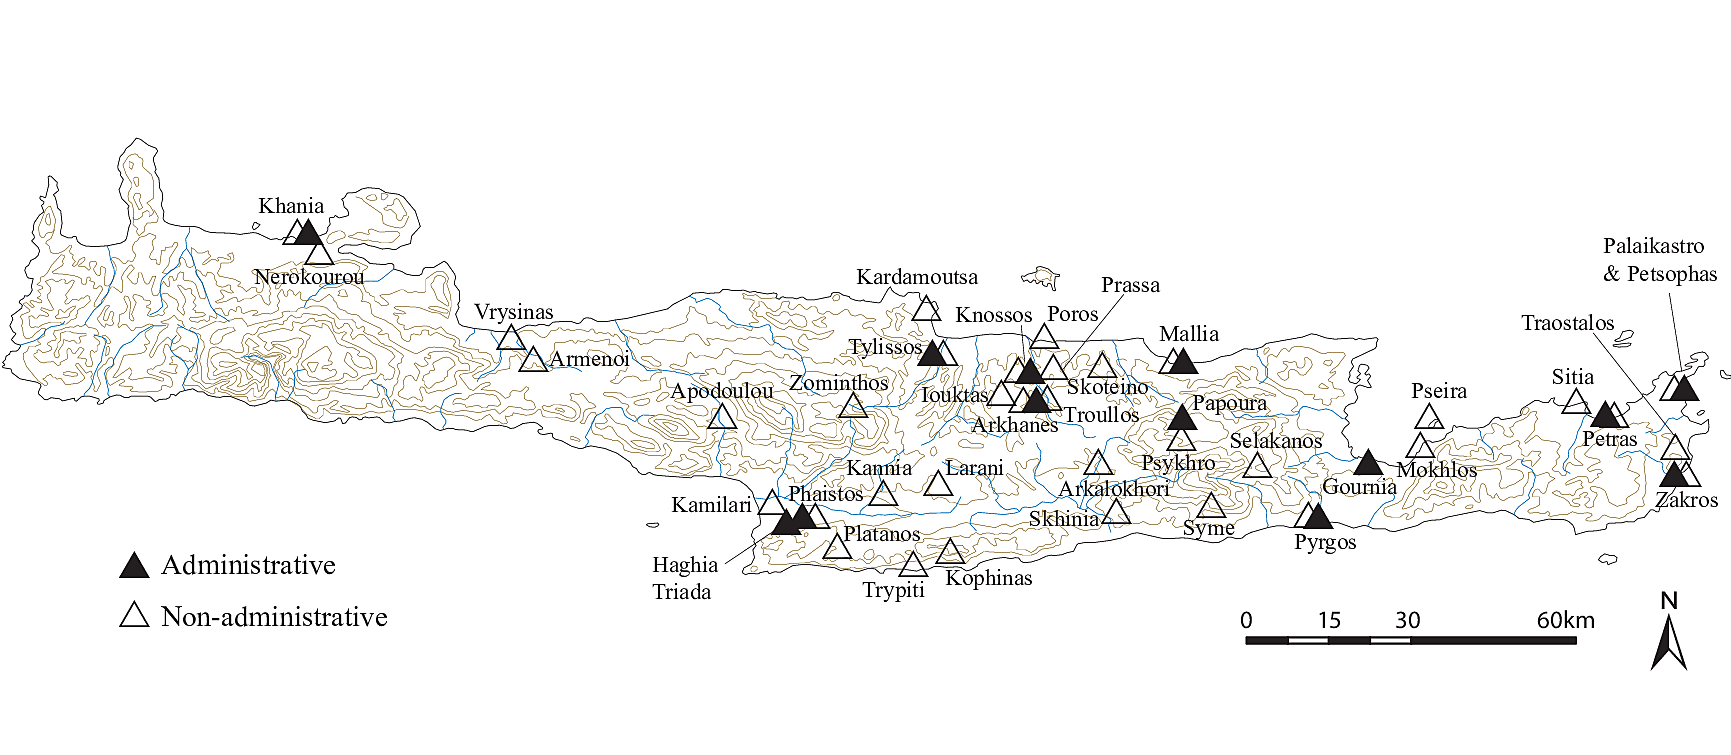
\includegraphics[width=0.8\textwidth]{Images/crete_LA.png} % Adjust width and filename
    \caption{Sites of Linear A fragments in Crete.\protect\footnotemark}
    \label{fig:crete_LA}
\end{figure}
\footnotetext{Figure \ref{fig:crete_LA} prepared by Yannis Galanakis and Ester Salgarella.}

Linear A was more widespread, covering completely Crete and the Aegean Islands and reaching the Greek mainland.
The main attestations of Linear A on the Greek mainland are very limited and generally considered sporadic and isolated. 
At Mycenae, a few Linear A inscriptions have been found, likely as a result of commercial or cultural exchanges with Crete. 
Similarly, some fragmentary finds have been uncovered at Tiryns, probably also related to trade or contacts with Minoan Crete.

\begin{figure}[H]
    \centering
    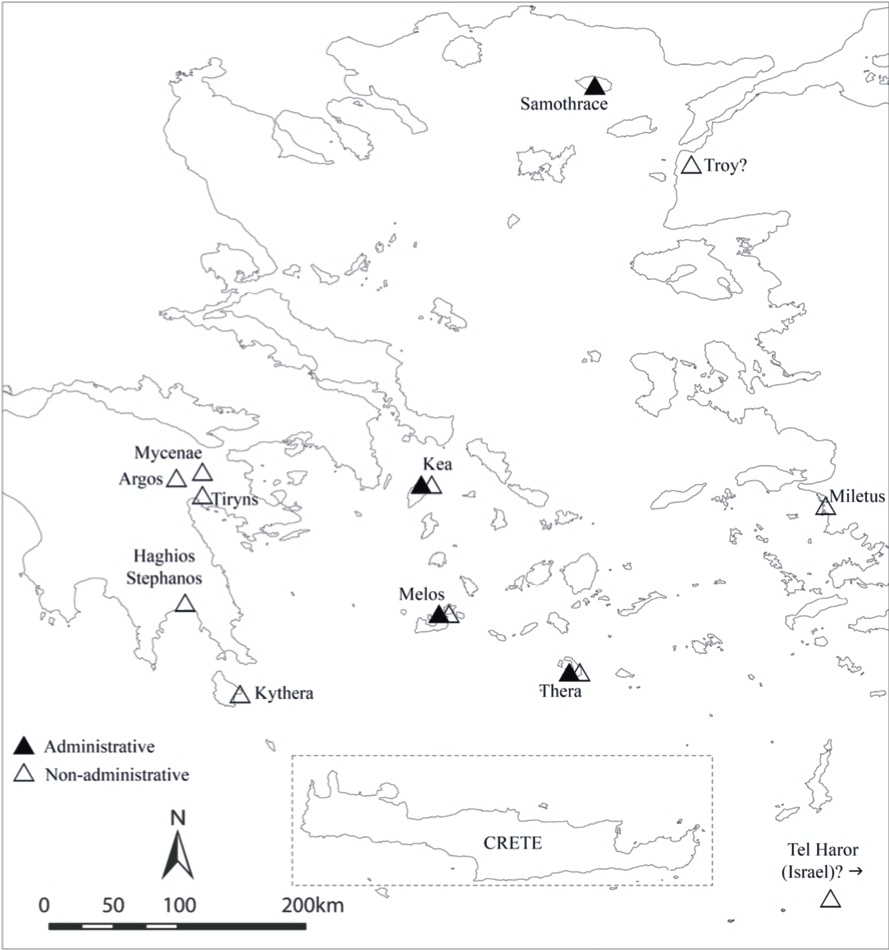
\includegraphics[width=0.8\textwidth]{Images/mainland_LA.jpg} % Adjust width and filename
    \caption{Sites of Linear A fragments in the Greek mainland.\protect\footnotemark}
    \label{fig:mainland_LA}
\end{figure}
\footnotetext{Figure \ref{fig:mainland_LA} prepared by Yannis Galanakis and Ester Salgarella.}

In contrast, Linear B is extensively attested on the Greek mainland, particularly in the Peloponnese, reflecting its administrative function during the Mycenaean period.
Major sites where Linear B documents have been found include Mycenae, Tiryns, Pylos, Thebes, and Athens.
Additionally, significant findings of Linear B tablets have been made in Crete, especially at Knossos and Khania.

The corpora of the two writing systems are relatively small, with Linear A consisting of approximately 1,400 documents, while Linear B comprises around 6,000 documents.
Another notable difference is that Linear A was more widely used for non-administrative purposes, particularly in religious contexts, whereas the number of non-administrative Linear B documents is considerably more limited. \cite{salg-ch1}


\begin{figure}[H]
    \centering
    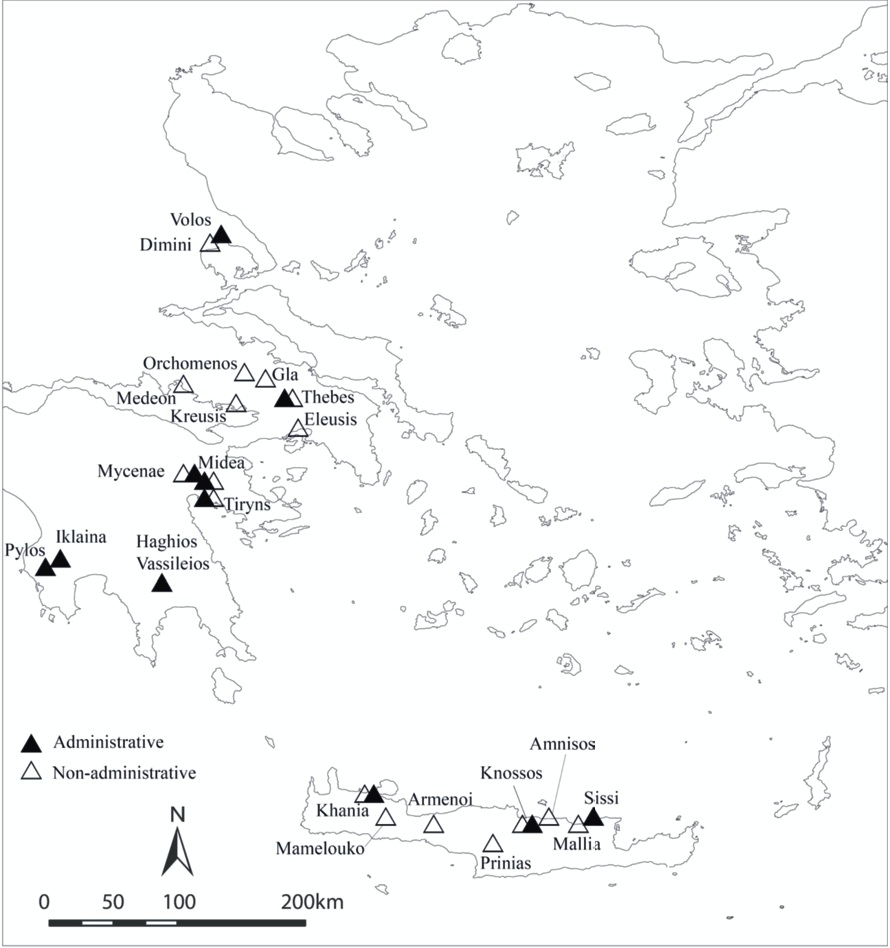
\includegraphics[width=0.8\textwidth]{Images/mainland_LB.jpg} % Adjust width and filename
    \caption{Sites of Linear B fragments in Crete and the Greek mainland.\protect\footnotemark}
    \label{fig:mainland_LB}
\end{figure}
\footnotetext{Figure \ref{fig:mainland_LB} prepared by Yannis Galanakis and Ester Salgarella.}


\section{Linguistic features}
The two writing systems are characterized by similar structural features, reflecting the connection between Linear A and Linear B and the derivation of the latter from the former.

The primary similarity between the two scripts lies in their syllabic structure, which constitutes a defining feature of both writing systems.
Both Linear A and Linear B are syllabic scripts, meaning that each symbol represents a syllable rather than an individual letter or a full word.
In addition to syllabic signs, both systems incorporate a set of logograms: symbols representing entire words or concepts.

This logographic component is particularly prominent in Linear A, where a significant number of signs are used to denote specific objects, actions, or concepts, often associated with administrative and religious contexts.
By contrast, Linear B employs a more restricted set of logograms, reflecting its primary function in administrative record-keeping.
Notably, the logograms used in Linear A were generally not inherited by Linear B, with a single exception: the logogram for "wool" (MA+RU), which is attested in both scripts.
However, the principles governing the formation of logograms remained unchanged, as in both scripts they are formed by juxtaposing or combining two or more signs, either horizontally or vertically.
\begin{figure}[H]
    \centering
    \begin{subfigure}[b]{0.6\textwidth}
        \centering
        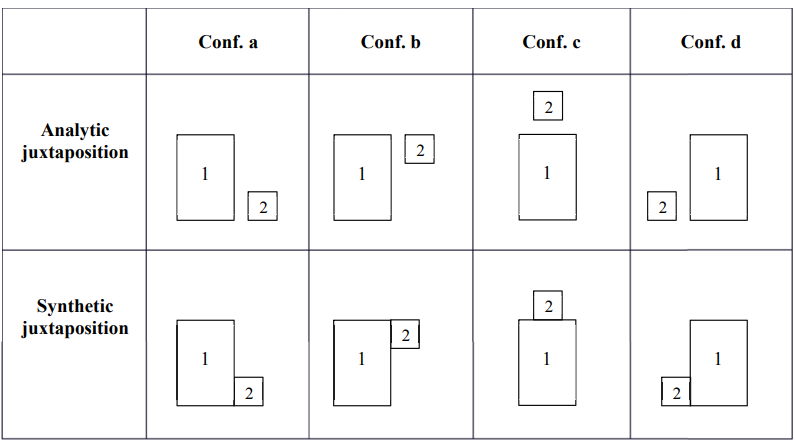
\includegraphics[width=\textwidth]{Images/logograms.png}
        \caption{Logogram construction criteria.}
        \label{fig:logograms}
    \end{subfigure}
    \hspace{0.05\textwidth}
    \begin{subfigure}[b]{0.3\textwidth}
        \centering
        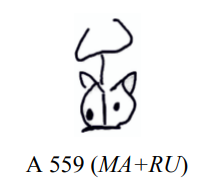
\includegraphics[width=\textwidth]{Images/ma-ru.png}
        \caption{LA logogram for wool.}
        \label{fig:ma-ru}
    \end{subfigure}
    \caption{Logograms in Linear A and Linear B.}
    \label{fig:linearA_sites}
\end{figure}

\begin{figure}[H]
    \centering
    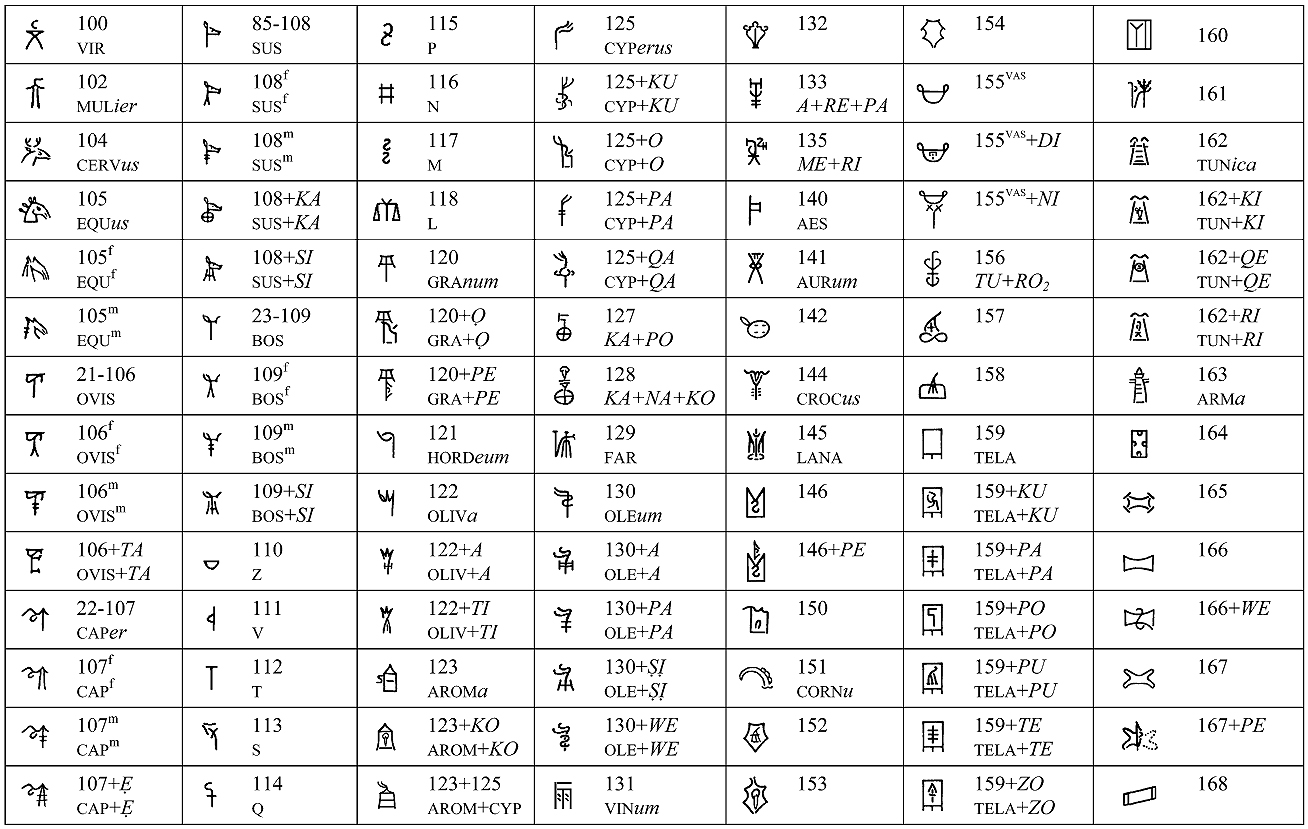
\includegraphics[width=1\textwidth]{Images/logos_1.jpg}
    \caption{Linear B logograms (symbols 100-168).}
    \label{fig:logos_1}
\end{figure}

Figure \ref{fig:logos_1} illustrates how logograms in Linear B can also incorporate syllabograms.
In these cases, the syllabogram is referred to as an adjunct and typically serves to qualify or specify the meaning of the logogram.
Moreover, the use of adjuncts is significantly more frequent in the Knossos corpus than on the Mainland, suggesting a possible continuity with Linear A, where isolated signs with sematographic value appear more commonly. \cite{salg-ch3}

Furthermore, a substantial portion of the Linear A syllabary is shared with Linear B, with approximately 72\% of Linear A signs being identical to those used in Linear B.
This overlap also illustrates continuity in symbol creation and in the assignment of phonetic values between the two systems.

\begin{figure}[H]
\centering
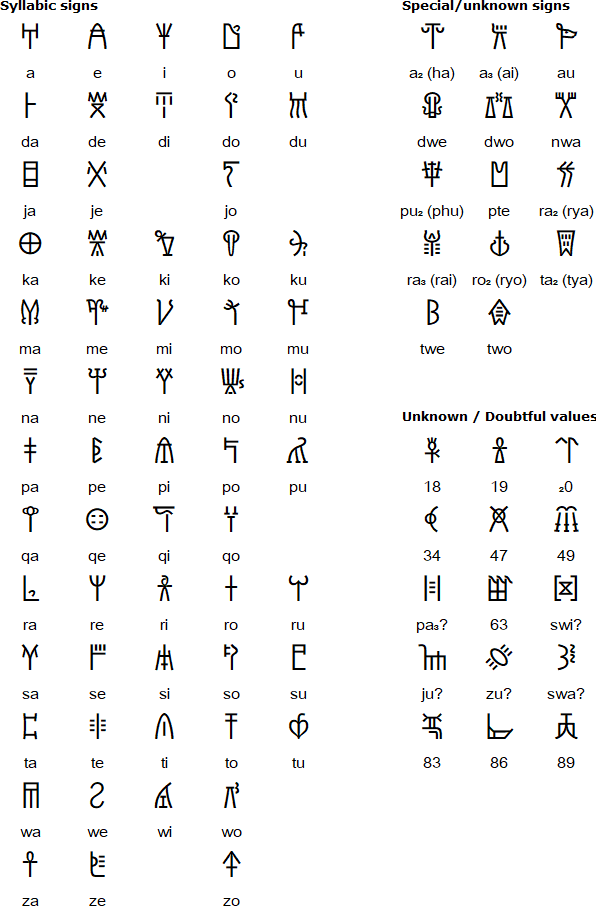
\includegraphics[width=0.8\textwidth]{Images/syll_LB.png}
\caption{All Linear B syllabograms with the associated phonetic values.}
\label{fig:syll_LB}
\end{figure}

As observed in Figure \ref{fig:syll_LB}, signs referring to the same vowel exhibit recurring patterns, a characteristic feature of syllabic scripts also evident in Linear A.
One of the most debated assumptions regarding the relationship between Linear A and Linear B is the principle of homomorphy and homophony.
This principle posits that signs which are visually similar (homomorphy) in both scripts also share the same phonetic value (homophony), representing the same syllable. \cite{salg-ch1}

This observation has led to the widely accepted conclusion that Linear A encodes a language fundamentally different from Linear B, with the latter used to represent an archaic form of Ancient Greek.
Consequently, although scholars are able to phonetically transcribe Linear A inscriptions, the language remains undeciphered and its meaning unknown. 

\section{The decipherment of Linear B} \label{sec:decipherment}
Ever since the discovery of the first Linear B tablets in 1900 by Sir Arthur Evans at Knossos, the script has been a subject of intense scholarly interest.
Evans himself introduced the classification of Aegean scripts that is still used today.
He also made the earliest attempts to decipher Linear B, though without success.

The breakthrough in understanding Linear B came after World War II, following major discoveries at the site of Pylos in 1939, which uncovered a large number of tablets and inscriptions.
A key figure in the decipherment of Linear B was Michael Ventris, a British architect and amateur linguist.
Ventris, in collaboration with philologist John Chadwick, succeeded in deciphering the script in 1952, demonstrating that it encoded an early form of Ancient Greek.

\subsection{The knowledge before the decipherment}

Before the decipherment of Linear B, scholars attempted to understand the script by studying it in isolation and by comparing it with known languages.  
One of the earliest hypotheses focused on the similarity between the Linear B syllabary and the Cypriot syllabary, a syllabic script used from about the eleventh to the fourth centuries BCE.  
The latter, which was also used to write an archaic form of Greek, shared a significant number of signs with Linear B.

However, this resemblance proved misleading in several respects.  
Although many signs appeared visually similar, as can be observed in Figure \ref{fig:lb-cypr}, their phonetic values often differed between the two systems.  
Moreover, the scripts treated grammatical suffixes differently.  
In Linear B, grammatical suffixes were frequently omitted, whereas this was not the case in the Cypriot syllabary, where the syllabogram "se" was regularly employed to indicate word endings.

Because "se" appeared regularly in the Cypriot syllabary but was rare in Linear B, early researchers concluded that Linear B could not represent the Greek language.  
In particular, Arthur Evans was convinced that the Minoan civilization was entirely distinct from the Mycenaean Greek world.  
This assumption, reinforced by Evans's authority and influence, contributed to delaying the recognition of the script's true linguistic nature. \cite{chad-ch2}

An example of this is the word "anthropos" (Ancient Greek: \textgreek{ἄνθρωπος}), which appears in Linear B as "a-to-ro-qo" (\textlinb{\Ba\Bto\Bro\Bqo}), while in Cypriot it is spelled with the "se" suffix as follows: "a-to-ro-po-se" (\textcypr{\Cse\Cpo\Cro\Cto\Ca}, written from right to left).

\begin{figure}[H]
\centering
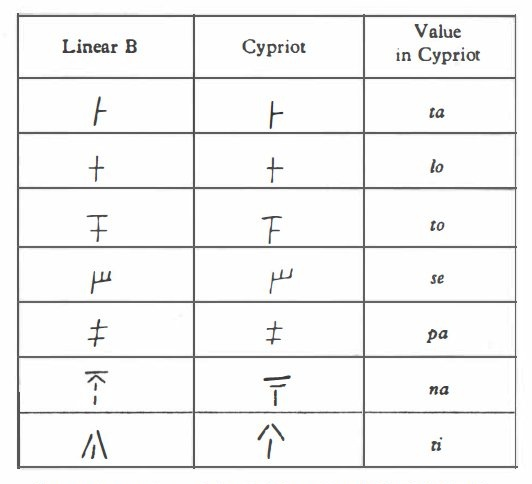
\includegraphics[width=0.6\textwidth]{Images/LB_cypriot.jpg}
\caption{Similarity between Linear B and Cypriot syllabary.}
\label{fig:lb-cypr}
\end{figure}

Evans had already established that most documents were administrative records.  
However, any attempt to decipher the script was hindered by unreliable underlying assumptions, while many aspects of the language remained unknown.

The most significant contribution came from Dr. Alice Kober, an American linguist. 
She was the first to approach the script methodically in order to uncover the nature of the underlying language.
She sought to answer fundamental questions, such as whether the language was inflected or whether specific forms were used to indicate gender and number.

Through her careful analysis, she was able to identify grammatical patterns, including distinctions between masculine and feminine nouns, as well as examples of inflection.
These results were achieved through a systematic study of repeated sign groups and their contexts, which she meticulously documented in her notebooks.
Her work challenged Evans's assumptions about the non-Greek nature of the language and paved the way for Ventris' later decipherment.
The outcome of her research was a set of "triplets", groups of three related words differing only in their endings, which provided critical evidence of an inflected language structure and were later referred to as "Kober's triplets".
Some examples of these triplets are shown in Figure \ref{fig:kobler_triplets}. \cite{chad-ch3}


\begin{figure}[H]
\centering
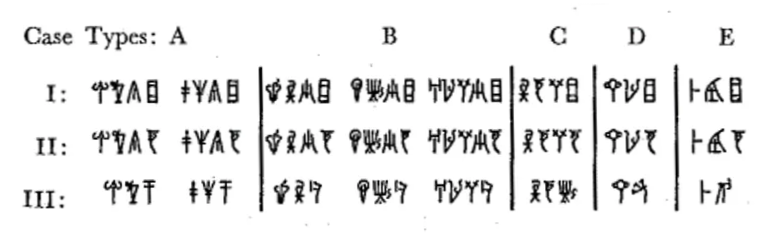
\includegraphics[width=0.8\textwidth]{Images/kobler_triplets.png}
\caption{Kobler's triplets examples.}
\label{fig:kobler_triplets}
\end{figure}

\subsection{The decipherment by Ventris and Chadwick} \label{subsec:ventris-chadwick}
The initial phase of the decipherment of Linear B involved the identification of numerical signs and easily recognizable logograms.
This preliminary work was largely accomplished by Sir Arthur Evans, who successfully identified the most frequently occurring logograms and reconstructed the basic features of the numerical system.
Notably, the Linear B script lacked a symbol for zero, but included fractional signs and was based on a decimal structure.

Building on these foundations, scholars began to assign tentative phonetic values to individual syllabograms through contextual analysis.
By examining recurring patterns and the placement of signs within administrative texts, it became possible to propose the phonetic values of certain symbols.
For instance, words such as "total" and "sons," which regularly appeared in similar tabular contexts, offered valuable clues for these early phonetic assignments.

However, the construction of a comprehensive and reliable grid of syllabograms was not feasible until the publication of the Pylos tablets in 1951.
This newly available corpus significantly expanded the body of evidence, enabling more systematic linguistic analysis.

Michael Ventris began his work on the decipherment in 1950, initially by circulating a questionnaire among scholars to gather views on the possible nature of the language encoded in Linear B and its potential relationship to Linear A or the Cypriot syllabary.

Realizing that scholarly opinion was divided, Ventris adopted a combinatorial and structural approach.
He explored positional patterns of signs within words, aiming to deduce their possible function or phonetic value.
By analyzing the frequency and distribution of certain symbols, particularly those likely to represent vowels, he was able to identify a subset of syllabograms corresponding to pure vowels.

A key breakthrough came from the identification of inflectional endings, many of which were made possible by the foundational work of Alice Kober.
Kober had demonstrated, through rigorous tabulation of sign groups, that the language encoded by Linear B exhibited an inflectional structure.
Ventris incorporated these findings into his research and began constructing a syllabic grid, updating it continually in light of new phonological rules and morphological patterns.

For example, he correctly identified the syllabogram \textlinb{\Bsi} as representing the syllable si, based on its frequent use in noun declensions and verb conjugations.
Its function mirrored that of the Ancient Greek suffix \textgreek{σι}, which appears in both oblique noun forms and verbal endings.

Additionally, place names proved particularly helpful, especially when accompanied by adjectival derivatives.
These offered valuable comparisons with known Greek toponyms and morphological structures.

As Ventris refined his hypotheses and incorporated increasingly sophisticated linguistic deductions, especially regarding inflectional patterns and suffixes, he was able to assign phonetic values to a majority of the signs.
Through this methodical approach, he successfully constructed a nearly complete syllabary grid.
Most of his assignments proved to be correct, with only minor exceptions that were later adjusted through collaborative efforts with John Chadwick and subsequent scholarly review. \cite{chad-ch4}

\begin{figure}[H]
\centering
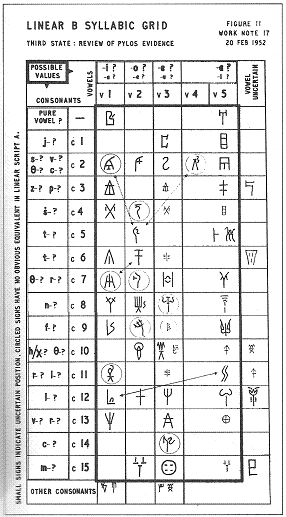
\includegraphics[width=0.8\textwidth]{Images/ventris_grid.png}
\caption{Ventris' syllabary grid.}
\label{fig:ventris_grid}
\end{figure}

Together, Ventris and Chadwick continued to investigate how the script encoded the phonology of the Mycenaean Greek language, recognizing that Linear B imposed structural constraints on how sounds were represented.
The syllabary, like many early writing systems, lacked a one-to-one correspondence with spoken Greek.
To better understand these adaptations, they analyzed the principles governing the script's orthography, namely how Greek words were transcribed within the limitations of the Linear B system.

The following rules summarize the most significant phonological and orthographic conventions that Ventris and Chadwick identified in the course of their research:

\begin{enumerate}
\item The script distinguishes five vowels: \textit{a, e, i, o, u}. Vowel length, however, is not indicated.

\item The second component of diphthongs ending in \textit{-u}, such as \textit{au, eu, ou}, is represented explicitly.

\item In diphthongs ending in \textit{-i} (e.g., \textit{ai, ei, oi, ui}), the second component is generally omitted, except:
\begin{itemize}
    \item when it occurs before another vowel, in which case it is represented as \textit{y};
    \item in the initial syllable \textit{ai}, where the full diphthong is retained.
\end{itemize}

\item Glides occurring between a front vowel and a following vowel are indicated:
\begin{itemize}
    \item the glide after \textit{i} is written as \textit{j};
    \item the glide after \textit{u} is written as \textit{w}.
\end{itemize}
These sounds are typically omitted in Greek alphabetic spelling.

\item The script represents twelve consonants:
\begin{itemize}
    \item \textbf{j}: used only to represent diphthongal \textit{i} or as a glide (see point 3);
    \item \textbf{w}: corresponding to the archaic Greek digamma (\textit{\textgreek{ϝ}}), pronounced as in English \textit{w};
    \item \textbf{d, m, n, s}: approximately as in later Greek and English;
    \item \textbf{r}: corresponding to Greek \textit{l} and \textit{r};
    \item \textbf{z}: corresponding to Greek \textit{z}; its exact phonetic value in Mycenaean Greek remains uncertain;
    \item \textbf{p, t, k}: representing both plain and aspirated stops, as the script does not distinguish aspiration;
    \item \textbf{q}: representing a series of labio-velar stops (\textit{kw, gw, khw}), which later disappeared from Greek but were preserved in Latin (e.g., \textit{quis}, \textit{unguem}).
\end{itemize}

\item The script does not represent aspiration; thus, aspirated consonants (\textit{ph, th, kh}) are not distinguished from their unaspirated counterparts.

\item The consonants \textit{l, m, n, r, s} are omitted when they occur:
\begin{itemize}
    \item at the end of a word;
    \item before another consonant.
\end{itemize}
For example, \textit{po-me} = \textit{poimen} (\textgreek{ποιμήν}) "shepherd"; \textit{ka-ko} = \textit{khalkos} (\textgreek{χαλκός}) "bronze"; \textit{pa-te} = \textit{pater} (\textgreek{πατήρ}) "father".

\item Initial \textit{s-} is generally omitted before another consonant.

\item In consonant clusters involving a stop + \textit{w}, both consonants are represented, with an intervening vowel that is either taken from the following syllable or supplied as a default. However, \textit{r} preceding \textit{w} is typically omitted.

\item Stop consonants (\textit{d, k, p, q, t}) occurring before another consonant are typically written with the vowel of the following syllable (less often the preceding syllable). 
For example:
\begin{itemize}
    \item \textit{ku-ru-so} = \textit{khrusos} (\textgreek{χρυσός}) "gold";
    \item \textit{A-mi-ni-so} = \textit{Amnisos} (\textgreek{Ἀμνισός}).
\end{itemize}
Special orthographic solutions are used to represent final consonant clusters, as in:
\begin{itemize}
    \item \textit{wa-na-ka} = \textit{wanax} (\textgreek{ϝάναξ}) "king".
\end{itemize}
\end{enumerate}

These conventions reveal the extent to which the Linear B script adapted to the phonology of Mycenaean Greek, despite being constrained by a syllabic system originally designed for a different language. \cite{chad-ch5}

The decipherment of Linear B was finally confirmed one year later, when in 1953 a new tablet found in Pylos could be translated only by using Ventris' grid.
This independent verification of the decipherment on material not previously available to Ventris provided undeniable evidence of his success. \cite{chad-ch6}

The work of Ventris and Chadwick, by combining structural analysis with comparative linguistics, thus not only unlocked the meaning of Linear B but also illuminated the phonological landscape of the earliest attested form of the Greek language.
\chapter{The cognate matching task}
As explained in Section \ref{sec:decipherment}, the decipherment of Linear B required a collective effort that involved several scholars and extended over multiple decades.

The main difficulties in any decipherment process concerning ancient languages arise from two factors: the absence of parallel texts that could guide the interpretation, and the extreme scarcity of surviving documents.
Even for domain experts, decipherment therefore demands encyclopedic linguistic and historical knowledge, combined with an enormous amount of manual work that is often prohibitive in terms of time and resources.
Moreover, the challenges encountered during the decipherment of one language are rarely reusable for others, since much of the required work and insights are closely tied to the specific features of that language and cannot be easily generalized \cite{luo}.
For example, the rules mentioned at the end of Section \ref{subsec:ventris-chadwick} are highly specific to the context of Linear B and its unique characteristics, and do not even apply to closely related scripts, such as Cypriot or possibly Linear A (for which no certainty exists, as the language remains undeciphered).

For these reasons, the introduction of computational methods and machine learning techniques has the potential to provide crucial assistance.
Nevertheless, the central obstacle remains the limited amount of training data.
This scarcity of examples makes it essential to design models that are able to learn effectively from small datasets and to generalize from minimal evidence.

In this respect, it is important to note that not all machine learning architectures are equally suitable for such low-resource conditions.
Transformers, for example, are a class of neural networks that have achieved remarkable results in modern natural language processing tasks, such as machine translation and text generation.
However, their success is strongly dependent on access to very large training corpora.
In the absence of such data, as is the case for ancient scripts, the application of transformers becomes impractical.
This explains why alternative architectures, which are better suited to scenarios where training data is scarce, are currently preferred in the computational study of ancient languages.

\section{Identifying Cognates}
Cognates are words in different languages that share a common etymological origin.
Identifying cognates is a crucial task in historical linguistics, as it allows researchers to trace the evolution of languages and to understand their relationships.
In the case of Linear B, the identification of cognates provided valuable correspondences between the syllabic script and the phonetic representations of Ancient Greek, which proved instrumental in the decipherment process.
Cognate matching was indeed a key aspect of Ventris' work, as he relied on clearly identifiable cognates to assign phonetic values to Linear B signs.
However, the task of identifying cognates is not always straightforward, since it requires a deep understanding of the historical and linguistic context of the languages involved.
In addition, several phonological transformations had taken place over time, including the differentiation of aspirated consonants and the loss of certain sounds once present in Linear B, such as the digamma ({\textgreek{ϝ}}) and the labio-velar consonant \textit{q}.

Below are some examples of cognates identified between Linear B and Ancient Greek:  

\begin{itemize}  
    \item \textlinb{\Ba\Be\Bti\Bto} (a-e-ti-to) $\rightarrow$ \textgreek{ἀέθιστος}, \textgreek{ἐθίζω} \\  
    This example shows how a Linear B sequence corresponds directly to a recognizable Greek adjective and verb.

    \item \textlinb{\Ba\Bdi\Bnwa\Bta} (a-di-nwa-ta) $\rightarrow$ \textgreek{Ἀδινϝᾶτας} \\  
    An instance where the Linear B syllabogram "nwa" reflects the presence of the digamma.

    \item \textlinb{\Be\Bma\Baii} (e-ma-ha) $\rightarrow$ \textgreek{Ἑρμᾶς}, \textgreek{Ἑρμαῖ}, \textgreek{Ἑρμαίας} \\  
    Illustrates a clear lexical link to Greek terms related to Hermes.

    \item \textlinb{\Bko\Bno\Bso} (ko-no-so) $\rightarrow$ \textgreek{Κνωσός}\\  
    A straightforward toponym, the name of the main Minoan palace site.

    \item \textlinb{\Bwo\Bno\Bqe\Bwa} (wo-no-qe-wa) $\rightarrow$ \textgreek{Φονοκέϝας}, \textgreek{Φονοκέϝαν} \\  
    Preserves traces of the digamma and labio-velar consonants.

    \item \textlinb{\Bwo\Bro\Bki\Bjo\Bne\Bjo} (wo-ro-ki-jo-ne-jo) $\rightarrow$ \textgreek{ϝοργιονείον}, \textgreek{Ὀργιονεῖος}, \textgreek{Ὀργίωνες} \\  
    A more complex example, relating to anthroponyms and associations.

    \item \textlinb{\Bqi\Bsi\Bpe\Be} (qi-si-pe-e) $\rightarrow$ \textgreek{ξίφεις}, \textgreek{ξίφη}, \textgreek{ξίφεα} \\  
    Reflects the Linear B representation of the Greek word for "sword."  

    \item \textlinb{\Bre\Bu\Bko\Bto\Bro} (re-u-ko-to-ro) $\rightarrow$ \textgreek{Λεῦκτρον}, \textgreek{Λεῦκτροι} \\  
    A toponym, attested both in Linear B and later Greek sources.

    \item \textlinb{\Bqo\Bu\Bqo\Bta} (qo-u-qo-ta) $\rightarrow$ \textgreek{Βουβώτας} \\  
    Demonstrates the phonetic evolution of labio-velar sounds.

    \item \textlinb{\Bqe\Bqi\Bno\Bme\Bna} (qe-qi-no-me-na) $\rightarrow$ \textgreek{γεγινώμενα}, \textgreek{γιγνόμενα} \\  
    A verbal form that shows continuity in Greek morphology.

    \item \textlinb{\Bpo\Bro\Bwi\Bto\Bjo} (po-ro-wi-to-jo) $\rightarrow$ \textgreek{πλωϝιστοῖο} \\  
    Example of a genitive form with preservation of the digamma.

    \item \textlinb{\Bpo\Bti\Bpi} (po-ti-pi) $\rightarrow$ \textgreek{Πόρτις}, \textgreek{Πόρτιφι} \\  
    Reflects a proper name with different Greek attestations.

    \item \textlinb{\Ba\Bri\Bqa} (a-ri-qa) $\rightarrow$ \textgreek{Ἄρισβας} \\  
    Example of an anthroponym preserving older consonantal values.

    \item \textlinb{\Bko\Bno} (ko-no) $\rightarrow$ \textgreek{Σκοῖνος} \\  
    Shows the addition of a consonant in Ancient Greek.
\end{itemize}  

\section{Datasets} \label{sec:datasets}
In this section, the process of gathering and preparing the datasets used in this study is described.
It is worth noting that I made several choices in order to create a clean and consistent dataset.
The main choices are the following:

\begin{itemize}
    \item All diacritics, accents, breathings, and iota subscripts were removed from Ancient Greek forms, resulting in a simplified text. For example \textgreek{ἀέθιστος} is represented as \textgreek{αεθιστος}.

    \item All instances of uppercase letters were converted to lowercase in order to normalize the data. For instance \textgreek{Κνωσός} is represented as \textgreek{κνωσος}.
    Note also that Linear B does not distinguish uppercase and lowercase.
    
    \item All instances of punctuation were removed.
    
    \item Linear B words were represented using their Latinized transcription.
    Therefore, the dataset contains the word \textlinb{\Bko\Bwo} as ko-wo instead of the original Linear B characters.

    \item The instances of digamma were inserted in a suitable position also in the Greek form, despite their disappearance from Classical Greek.
    For example, the word \textgreek{κόρος} is represented as \textgreek{κορfος} in the dataset.
    In some cases, the version without digamma is also included, as in \textgreek{κουρος}.

    \item The only additional symbol employed, besides the standard Greek alphabet, is "h", used to represent the aspiration conveyed by the syllabogram \textlinb{\Baii} (ha).
    For instance, \textlinb{\Ba\Bpi\Baii\Bro} (a-pi-ha-ro) is rendered as \textgreek{αμφιhαλος}.
\end{itemize}

The sources of all the data included in the final version of the dataset are the following:

\begin{itemize}
\item \textbf{Luo's dataset} \cite{luo}: a collection of cognates between Linear B and Ancient Greek, compiled by Jiaming Luo. It contains 919 Linear B words together with their proposed Ancient Greek correspondences.
\item \textbf{Chris Tselentis' *Linear B Lexicon*} \cite{tselentis}: a lexicon comprising 1338 Linear B entries with Ancient Greek equivalents. A substantial portion of these entries overlap with Luo's dataset.
\item \textbf{Ventris and Chadwick's Vocabulary} \cite{chadwick-notes}: a digitized compilation based on the original notes and lexical work of Michael Ventris and John Chadwick, later supplemented with commentary by other scholars. The resource, available as a CSV file at \url{https://linear-b.kinezika.com/lexicon.html}, comprises 2747 unique words.
It is organized as a vocabulary, offering definitions and interpretative remarks on the terms, and thus represents an extended digital derivative of their foundational work.
\end{itemize}

\subsection{Prompt engineering}
Some tasks were automated using prompt engineering techniques with Gemini~2.0~Flash and Gemini~2.5~Flash, which proved effective for text processing and data manipulation. Whenever these techniques are employed, I explicitly indicate their use and summarize the prompt instructions that were critical to the task.
In general, the prompts followed these principles:

\begin{itemize}
\item \textbf{Clarity and specificity:} Clear, unambiguous instructions to reduce variance and align outputs with task requirements \cite{prompting-programming}.

\item \textbf{Iterative refinement:} Prompts were refined based on model outputs to improve quality across iterations.

\item \textbf{Contextualization:} Task-relevant context (e.g., field definitions, examples) was included to guide disambiguation.

\item \textbf{Structured reasoning:} Prompts encouraged stepwise reasoning for complex tasks (e.g., breaking a problem into sub-steps), leading to more coherent outputs \cite{cot}.

\item \textbf{Structured formatting:} Outputs were requested in explicit schemas (XML/JSON, bullet/numbered lists) to ensure machine-readable, post-processable results.

\item \textbf{Salience cues (including UPPERCASE for emphasis):} Key requirements were emphasized to prioritize the most important aspects and reduce omission errors \cite{uppercase-is-all-you-need}.
\end{itemize}

When necessary, I adjusted the model's generation settings to favor determinism: the \texttt{temperature} was set low (e.g., 0.1--0.3) to reduce randomness and increase repeatability, and \texttt{top-k} was fixed at 1 (greedy selection).

\subsection{Luo's Dataset}
Luo's dataset is the one on which the creator of the NeuroDecipher model (introduced later) tested its performance.
The model achieves excellent results on this dataset, reaching an accuracy of 84.7\% of cognates correctly matched \cite{luo}.

However, the dataset is not without limitations.
The main issue I identified upon closer inspection is that some proposed Greek cognates are not attested in extant Ancient Greek sources, but rather tentative transliterations of Linear B forms or artificially modified versions of Greek correspondences.
While this may artificially improve the cognate matching task, it does not reflect a realistic linguistic scenario and makes the dataset unsuitable for use in an automatic translation pipeline.
A few illustrative examples are given below:

\begin{itemize}
\item \textlinb{\Bqo\Bo} (qo-o) is correctly associated with \textgreek{βους}, as also confirmed by Tselentis' lexicon \cite{tselentis}. However, the dataset additionally lists \textgreek{κfοος}, which does not correspond to any attested Ancient Greek form.
\item \textlinb{\Bto\Bo} (to-no) is linked to \textgreek{θρονος}, likewise confirmed by Tselentis' lexicon \cite{tselentis}, but the dataset also includes \textgreek{θορνος}, an unattested form that results from an unjustified inversion of letters.
This error extends to \textlinb{\Bto\Bro\Bno\Bwo\Bko} (to-ro-no-wo-ko), where the listed cognate is \textgreek{θορνοfοργος}. I corrected this instead to \textgreek{θρονοfοργος} and \textgreek{θρονοfεργος}, both plausible formations obtained by combining \textgreek{θρόνος} ("throne, chair") with the productive suffix derived from \textgreek{ἔργον} ("work, deed"). The resulting compound restores the original sense of the term as "chair-maker" or "craftsman of thrones."
\item In several cases, the dataset conflates distinct gendered forms by grouping them under a single entry. For example, \textlinb{\Bne\Bwa} (ne-wa), corresponding to \textgreek{νεfα} or \textgreek{νεα}, feminine, and \textlinb{\Bne\Bwo} (ne-wo), corresponding to \textgreek{νεfος} or \textgreek{νεος}, masculine, were all grouped under \textlinb{\Bne\Bwa}, despite both variants being independently attested in the Linear B corpus.
\end{itemize}

The adjustments described above were applied to Luo's dataset in order to enhance its reliability and linguistic accuracy.
This revised version was then used both to measure the performance of the NeuroDecipher model on a more realistic dataset and as the foundation for constructing the final comprehensive dataset, which also integrates additional material from Tselentis' Linear B Lexicon and from the digitized vocabulary of Ventris and Chadwick.
The resulting revised dataset comprises 976 Linear B entries paired with their respective Ancient Greek correspondences.

\subsection{Tselentis' Dataset}
Tselentis' dataset represents a valuable resource for the study of Linear B, as it comprises a comprehensive lexicon of Linear B terms and their corresponding Ancient Greek forms.
It serves as a crucial reference point for validating and enriching the cognate pairs identified in Luo's dataset.

The main drawback of Tselentis' lexicon is that it was only available as a PDF document, which made it necessary to manually transcribe the entries into a more usable format.
After using an online OCR tool to extract its content into a CSV file, followed by targeted cleaning, a structured file containing all the fields in the lexicon was obtained.

Nevertheless, the data still required further processing to extract the Greek and Linear B forms in accordance with the normalization criteria outlined at the start of this section.
Several parsing mistakes, along with inconsistencies in accents, diacritics, and formatting, had to be corrected to ensure accuracy and consistency.
To streamline this process, Prompt Engineering techniques were employed with Gemini~2.0~Flash, guided by explicit processing directives.

These techniques enabled the automated correction of recurrent errors and inconsistencies, significantly accelerating data preparation.
The processed dataset was then reviewed manually to ensure its quality and reliability before integration into the final comprehensive dataset.

For transparency and repeatability, I detail here the precise directives provided to Gemini for dataset processing.

\bigskip
\noindent\textbf{PROCESSING RULES FOR LINEAR B TO GREEK COGNATES:}

\begin{enumerate}[label=\textbf{\arabic*.}, leftmargin=2.5em]
\setcounter{enumi}{-1}

\item CRITICAL: DO NOT MAKE ANY MODIFICATION TO GREEK COGNATES OR LINEAR B SEQUENCES IF THE MODIFICATION IS NOT MENTIONED IN THE FOLLOWING RULES! DO NOT CHANGE THE INPUT IN ANY POSSIBLE WAY AND ONLY APPLY THE GIVEN MODIFICATION RULES! NO FANTASY JUST BLINDLY OBEY!

\item SPLITTING MULTIPLE WORDS: When Linear B field contains multiple words separated by "/", create separate JSON objects for each word, matching with the corresponding Greek cognate in the same position.

\item HANDLING PARENTHESES: For Linear B words with parenthetical elements like "po-ni-ke-(j)a", create two separate entries (one with and one without the parenthetical element, like "po-ni-ke-ja" and "po-ni-ke-a").

\begin{enumerate}[label*=\textbf{\arabic*.}, leftmargin=2em]
  \item HANDLING PARENTHESES FOR GREEK COGNATE: if a word is presented with optional greek characters with parenthetical elements like "\textgreek{αιξμά(ν)ς}", include both variants with and without the letter in parentheses.
  \item HANDLING PARENTHESES FOR GREEK COGNATE: if a word is presented within parentheses, include it regardless, like "\textgreek{Αιθαλεύσι(Αιθαλεύς)}".
\end{enumerate}

\item MULTIPLE TRANSLATIONS: If a Linear B word has multiple possible Greek cognates, include all of them as an array within the same JSON object.

\item REMOVING DIACRITICS: Remove all accents, breathing marks, and other diacritics from Greek cognates.

\item HANDLING "ha" SIGN: When "ha" appears in Linear B, ensure the corresponding Greek cognate includes "h".

\item DIGAMMA CONVERSION: Convert every instance of digamma "F" to lowercase "f" in Greek cognates.

\item CRITICAL: ALLOWED CHARACTERS: Use ONLY these characters in Greek cognates: \textgreek{fhαβγδεζηθικλμνξοπρςστυφχψω}. DO NOT USE ANY OTHER CHARACTER FOR ANY REASON!

\item DISALLOWED CHARACTERS: Drop cognates containing disallowed characters, but preserve valid cognates found within parentheses or other markers.

\item IN SOME VERY RARE AND PARTICULAR CASES some cognates may be considered as DUBIOUS, IF AND ONLY IF THEY CONTAIN A LIKELY WRONG TRANSLITERATION AND A CORRECT MATCH IS ALREADY PRESENT. Put them in the "dubious" field, another optional array field in the JSON object.

\item if white spaces are present between syllables separated by - in the linear b sequence, remove them.

\item DO NOT USE PARENTHESES IN THE LINEAR B SEQUENCES OR IN THE GREEK COGNATE.
\end{enumerate}

Applying these directives reduced OCR noise and errors, preserving valid cognate pairs while preventing format drift that would hinder downstream parsing.
These directives, together with a number of examples and some input and output definitions, allowed me to automate most of the manual work that the data needed in order to be ready to use.

\subsection{Brute-Force Cognate Extraction}

To enlarge the dataset, I implemented and applied a brute-force, syllabogram-aware matcher over a large Greek lexicon (composed by the Iliad and Odyssey).
Greek forms were first normalized (diacritics removed, lowercased) and then latinized via a direct character map aligned to Linear B conventions (e.g., \textgreek{ξ} $\rightarrow$ \textit{ks}); 
special cases included the digamma (\textgreek{ϝ} with later re-insertion of f/h during reconstruction) and the
labio-velar \textit{q} (permitted to align with $\{q,p,k\}$).

\paragraph{Matching logic.}
Each Linear B form is tokenized into syllabograms and compared against every latinized Greek word by
scanning both sequences left-to-right and greedily aligning syllabograms to characters.
The matcher handles three syllabogram classes, with tailored rules:
\begin{itemize}[leftmargin=2em]
  \item \textbf{V (length 1):} align the same vowel; mismatches advance the Greek pointer (counted as a skip).
  \item \textbf{CV (length 2):} align the initial consonant and then the vowel; special handling covers clusters
        such as \textit{k}+\textit{s} that straddle the next syllable (e.g., \textit{ks}).
  \item \textbf{Specific triads (length 3):} a small set of syllabograms (e.g., \textit{phu}) is matched as a fixed mini-pattern.
\end{itemize}

\paragraph{State tracked during scanning.}
The algorithm maintains (i) the total number of skipped Greek characters and the maximum consecutive
skip streak (to avoid over-skipping), (ii) a flag for illegal syllable mappings, and (iii) a small
relaxation allowing a single liquid glide (e.g., an isolated ``r'').

\paragraph{Acceptance gates.}
After the pass, a candidate pair is accepted only if all of the following hold:
\begin{enumerate}[label=(\roman*), leftmargin=2em]
  \item near-complete coverage of the Linear B syllables, i.e.\ the pointer must reach the last or penultimate syllable;
  \item the Greek pointer must lie within three characters of the word's end;
  \item the total number of skips must be fewer than four and no more than two consecutive characters may be skipped;
  \item an initial-character compatibility heuristic holds (to avoid wild misalignments);
  \item no illegal syllable mapping was flagged;
  \item for short Linear B words, stricter thresholds are applied (fewer allowed skips and a smaller tail).
\end{enumerate}

\paragraph{Outputs and design choice.}
For each accepted pair, the algorithm records a coverage score,
\[
\text{coverage} \;=\; \frac{\text{matched syllables}}{\text{total syllables}},
\]
and reconstructs the Greek surface form by re-inserting any f/h positions suppressed during normalization.
The overarching design targets recall over precision: collect as many plausible pairs as possible, even at the cost of some spurious matches, to be filtered later.

\begin{lstlisting}[language=Python, caption=Brute-Force matching algorithm, breaklines=true, postbreak=\mbox{\hspace{50pt}\textcolor{red}{$\hookrightarrow$}\space}]
def match(lin_b_words, greek_words):
    for lb_word in lin_b_words.keys():  # scan each Linear B entry
        lb_syllables = lb_word.split("-") # LB sequence to syllables
        for gr_word in greek_words.keys(): # scan each Greek candidate

            gr_chars = list(gr_word) # Greek word to char list
            i_syl = 0 # index over LB syllables
            j_chr = 0 # index over Greek chars
            skip_count = 0 # total skipped Greek chars
            skip_streak = 0 # current consecutive skips
            max_skip_streak = 0 # max consecutive skips seen
            invalid_syllable = False # flag for invalid syllable mapping
            skipped_syllables = [] # track skipped syllables if needed

            while i_syl < len(lb_syllables) and j_chr < len(gr_chars):
                lb_syllable = lb_syllables[i_syl]
                gr_char = gr_chars[j_chr]

                if len(lb_syllable) == 1:
                    if gr_char == lb_syllable:
                        skip_streak = 0
                        i_syl += 1
                        j_chr += 1
                    else:
                        skip_count += 1
                        skip_streak += 1
                        if skip_streak > max_skip_streak:
                            max_skip_streak = skip_streak
                        j_chr += 1

                elif len(lb_syllable) == 2:
                    cons = lb_syllable[0]

                    if cons == "k":
                        has_room = (j_chr + 2) < len(gr_chars)
                        tail = gr_chars[j_chr + 1 : j_chr + 3]
                        # checks double guttural
                        has_dg = has_room and ("".join(tail) == lb_syllable)

                        if gr_char == "k" and not has_dg:
                            skip_streak = 0

                            has_next_char = (j_chr + 1) < len(gr_chars)
                            # checks ks
                            next_is_s = has_next_char and (gr_chars[j_chr + 1] == "s")
                            has_next_syl = i_syl < (len(lb_syllables) - 1)

                            if next_is_s and has_next_syl:  # matched ks
                                next_syl = lb_syllables[i_syl + 1]
                                if next_syl[0] == "s":
                                    i_syl += 2
                                    j_chr += 2
                                    vowel_ok = (
                                        j_chr < len(gr_chars)
                                        and next_syl[1] == gr_chars[j_chr]
                                    )
                                    if vowel_ok:
                                        j_chr += 1
                                else:
                                    i_syl += 1
                                    j_chr += 1
                                    vowel_ok = (
                                        j_chr < len(gr_chars)
                                        and lb_syllable[1] == gr_chars[j_chr]
                                    )
                                    if vowel_ok:
                                        j_chr += 1
                            else:
                                i_syl += 1
                                j_chr += 1
                                vowel_ok = (
                                    j_chr < len(gr_chars)
                                    and lb_syllable[1] == gr_chars[j_chr]
                                )
                                if vowel_ok:
                                    j_chr += 1
                        else:
                            j_chr += 1
                            skip_count += 1
                            skip_streak += 1
                            if skip_streak > max_skip_streak:
                                max_skip_streak = skip_streak

                    if cons == "q":  # labio-velar mapped to {q,p,k}
                        is_labio_map = gr_char in ("q", "p", "k")
                        if is_labio_map:
                            skip_streak = 0
                            i_syl += 1
                            j_chr += 1
                            vowel_ok = (
                                j_chr < len(gr_chars)
                                and lb_syllable[1] == gr_chars[j_chr]
                            )
                            if vowel_ok:
                                j_chr += 1
                        else:
                            j_chr += 1
                            skip_count += 1
                            skip_streak += 1
                            if skip_streak > max_skip_streak:
                                max_skip_streak = skip_streak
                    ...
                if len(lb_syllable) == 3:
                    if lb_syllable == "phu":
                        has_u = ((j_chr + 1) < len(gr_chars)) and (gr_chars[j_chr + 1] == "u")
                        if gr_char == "p" and has_u:
                            skip_streak = 0
                            i_syl += 1
                            j_chr += 2
                        else:
                            j_chr += 1
                            skip_count += 1
                            skip_streak += 1
                            if skip_streak > max_skip_streak:
                                max_skip_streak = skip_streak
                    ...

            # allow single liquid glide
            if max_skip_streak == 2 and len(skipped_syllables) == 1:
                if skipped_syllables[0][0] == "r":
                    max_skip_streak = 0

            # --- Acceptance constraints ---
            start_ok = (
                lb_word[0] == gr_word[0]
                or (lb_word[0] == "p" and gr_chars[0] == "p")
                ...
            )
            lb_aligned = i_syl >= (len(lb_syllables) - 1)
            gr_near_end = j_chr >= (len(gr_word) - 3)
            skips_ok = skip_count < 4
            streak_ok = max_skip_streak <= 2
            mapping_ok = not invalid_syllable

            conds1 = (lb_aligned, gr_near_end, skips_ok, start_ok, streak_ok, mapping_ok)
            gate1 = all(conds1)

            short_lb = len(lb_syllables) <= 3
            near_end_tight = j_chr >= (len(gr_word) - 2)
            short_ok = (skip_count <= 2) and near_end_tight and (max_skip_streak < 2)
            # conditions for shorter LB words
            gate2 = (short_lb and short_ok) or (not short_lb)

            if gate1 and gate2:
                # Reconstruct normalized Greek, re-inserting 'f'/'h'
                greek_norm_chars = list(greek_words[gr_word])
                dropped = len(greek_words[gr_word]) < len(gr_chars)
                if dropped:
                    fh = ("f", "h")
                    positions = [p for p, c in enumerate(gr_chars) if c in fh]
                    for off, pos in enumerate(positions):
                        greek_norm_chars.insert(pos + off, gr_chars[pos])

                coverage = i_syl / len(lb_syllables)
                match_pair = ("".join(greek_norm_chars), coverage)
                lin_b_words[lb_word]["cognates"].append(match_pair)

    return lin_b_words
\end{lstlisting}

The brute-force search has complexity $O(N_{\text{LB}} \cdot N_{\text{GR}} \cdot L)$, where $N_{\text{LB}}$ is the number of Linear B forms, $N_{\text{GR}}$ is the number of Greek forms, and $L$ is the maximum length of words.
For the translation dataset, $N_{\text{LB}} = 4809$ and $N_{\text{GR}} = 18646$, with $L \leq 19$, as the longest word is \textlinb{\Ba\Bni\Bja\Be\Be\Bro\Bpa\Bjo\Bqe\Bro\Bsa} (a-ni-ja-e-e-ro-pa-jo-qe-ro-sa).

\paragraph{Outputs refinement.}
Clearly, this brute-force approach is not perfect and, while it attempts to filter out very different words as much as possible, it inevitably returns more pairs than true cognates.
This limitation is acceptable because a second filtering stage prunes and re-ranks candidates by means of prompt engineering.
The filter is driven by a structured XML prompt and produces a strict JSON response. The main instructions given to Gemini~2.5~Flash can be summarized as follows:

\begin{itemize}[leftmargin=2em]
  \item \textbf{Invocation of Luo's principles}: the model must evaluate each proposal against the four cognate matching principles, which will be detailed in the next section, ensuring that they are applied consistently and rigorously.
  These principles are distributional similarity of matching characters, monotonic character mapping within cognates, structural sparsity of cognate mapping, and significant cognate overlap within related languages.
  \item \textbf{Character policy}: enforce the restricted output alphabet for Ancient Greek forms introduced in Section \ref{sec:datasets}, disallowing accents, breathings, or subscript iota.
  \item \textbf{Phonological mapping tables}: require adherence to explicit Linear B $\rightarrow$ Ancient Greek correspondence tables for consonants and vowels, supported by contextual notes (e.g. treatment of labiovelars, liquids, or clusters).
  \item \textbf{Independence from hints}: all provided "proposed cognates" are treated as non-binding; the model must search beyond them and consider the broader Ancient Greek corpus.
  \item \textbf{Plausibility assessment}: evaluate candidates against a rubric of evaluation criteria, aligned with the four principles, and reject items that fail any check.
  \item \textbf{Reasoning scaffold}: follow an explicit five-step chain-of-thought structure to ensure consistency in the decision path: syllabogram analysis $\rightarrow$ monotonicity enforcement $\rightarrow$ sparsity audit $\rightarrow$ pattern comparison $\rightarrow$ composite ranking.
  \item \textbf{Calibration of likelihoods}: apply a calibrated numerical scale with illustrative examples ranging from well-attested to speculative cases, so that likelihood scores are interpretable and comparable across words.
  \item \textbf{Automatic downweighting and hard caps}: apply four penalties, for example, $-0.3$ for three or more non-trivial transformations or any reordering; $-0.2$ for rarity, conflict with scholarship, or semantic stretch, and enforce global caps: likelihood $<0.7$ whenever the Linear B sequence contains unknown syllabograms such as *19, and $<0.85$ for novel, unattested proposals even if other checks are passed.
  \item \textbf{Worked examples}: provide a wide set of input-output examples illustrating common patterns (such as $q{+}s$, digamma insertion, or suffixal transformations) to calibrate the model's application of rules and character policy.
  \item \textbf{Quality-control gate}: prefer fewer, higher-quality outputs over speculative additions and abstain when uncertain.
  \item \textbf{Instance metadata}: input word block: Linear B form, completeness level, optional definition from Chadwick and Ventris' vocabulary \cite{chadwick-notes}, any pre-proposed cognates with their brute-force matching scores, and entity type, to give context without constraining the final choice.
\end{itemize}

The complete XML prompt and the exact JSON schema are presented in the source code repository.
After this automated filtering stage, the dataset was manually reviewed to ensure the quality and reliability of the final cognate pairs.
Additionally, some cognates pairs were added from Ventris and Chadwick's vocabulary \cite{chadwick-notes} when they were missing from the previous datasets.

\section{Cognate Matching Model}
In this section, the architecture and training procedure of the cognate matching model created by Jiaming Luo \cite{luo} are described.
The model is based on a sequence-to-sequence (seq2seq) architecture with attention mechanisms, which has been shown to be effective for various natural language processing tasks, including machine translation and text generation.
The model is trained to take a Linear B word as input and generate its corresponding Ancient Greek cognate as output.
As explained in Luo's paper, the main challenge of the decipherment task is the lack of a strong supervision signal that guides standard machine translation algorithms.
To address this challenge, he proposed an architecture that learns patterns of language transformation.
Moreover, the model is designed to be language-agnostic, meaning that it can be applied to other decipherment tasks beyond Linear B and Ancient Greek.
In order to achieve this, the model relies on a set of principles that capture the general characteristics of cognate relationships between languages.

\subsection{Cognate Matching Principles}
The four principles that guide the model's architecture and training are the following:
\begin{enumerate}[leftmargin=2em, label=\textbf{\arabic*.}]
    \item \textbf{Distributional similarity of matching characters:}
    matching characters are expected to appear in similar places in corresponding cognates, therefore their local context should match as well.

    \item \textbf{Monotonic character mapping within cognates:}
    cognates are expected to exhibit largely monotonic alignments, as character reorderings are rare.

    \item \textbf{Structural sparsity of cognate mapping:}
    cognate matchings are expected to be sparse and near one-to-one between segments derived from the same proto-origin.

    \item \textbf{Significant cognate overlap within related languages:}
    it is assumed that the derived vocabulary will provide sufficient coverage for recovering lost cognates.
\end{enumerate}

\subsection{The Generative Framework} \label{sec:generative-framework}
The model architecture relies on a latent variable $\mathcal{F}=\{f_{ij}\}$, representing the word-level alignment between the words in the lost language $\mathcal{X}=\{x_i\}$ and the known language $\mathcal{Y}=\{y_j\}$.
The following joint probability is derived:
\[
\mathbf{P}(\mathcal{X}, \mathcal{Y})
= \sum_{\mathcal{F}\in \mathbb{F}}
  \mathbf{P}(\mathcal{F})\,\mathbf{P}(\mathcal{X}\mid \mathcal{F})\,\mathbf{P}(\mathcal{Y}\mid \mathcal{F}, \mathcal{X})
\propto
\sum_{\mathcal{F}\in \mathbb{F}}
  \mathbf{P}(\mathcal{Y}\mid \mathcal{X}, \mathcal{F})
=
\sum_{\mathcal{F}\in \mathbb{F}}
  \prod_{y_j\in \mathcal{Y}}
  \mathbf{P}(y_j \mid \mathcal{X}, \mathcal{F}) \, ,
\]
where a uniform prior is assumed for $\mathbf{P}(\mathcal{F})$ and $\mathbf{P}(\mathcal{X}\mid \mathcal{F})$, and independence and identical distribution (i.i.d.) are assumed across $y_j\in\mathcal{Y}$.
Here, $\mathbb{F}$ denotes the set of all valid values of the latent variable $\mathcal{F}$.

The conditional probability $\mathbf{P}(y_j \mid \mathcal{X}, \mathcal{F})$ is further decomposed as:
\[
\mathbf{P}(y_j \mid \mathcal{X}, \mathcal{F})
= \sum_{x_i\in \mathcal{X}} f_{ij}\cdot \mathbf{P}_{\theta}(y_j \mid x_i) \, ,
\]
where $\mathbf{P}_{\theta}(y_j \mid x_i)$ is a neural seq2seq model with parameters $\theta$ that generates $y_j$ given $x_i$.
In this framework, the latent variable $\mathcal{F}$ captures the alignment between the two languages, incorporating the global constraints described by Properties 3 and 4, while the neural model learns to generate cognates based on character-level constraints defined in Properties 1 and 2.
However, directly optimizing the joint probability is infeasible, as it requires summing over all possible values of $\mathcal{F}$.
To overcome this issue, Luo adopted an Expectation-Maximization (EM) iterative training algorithm: the neural model is trained in the M-step to maximize the likelihood of $\prod_{y_j\in \mathcal{Y}} \mathbf{P}(y_j \mid \mathcal{X}, \mathcal{F})$ given fixed $\mathcal{F}$, while in the E-step $\mathcal{F}$ is estimated via a minimum-cost flow problem defined over the trained neural network.

\subsection{NeuroDecipher Model}
The neural model $\mathbf{P}_{\theta}(y_j \mid x_i)$, named NeuroDecipher, is based on a standard seq2seq architecture.
The three main components of the model are the encoder, the decoder, and the attention mechanism.

\paragraph{Encoder.}
The encoder consists of a stack of two embedding layers and a bidirectional LSTM.
This design enforces the requirement that character embeddings of the two languages reside in the same space, the Universal Character Embedding Space.
This is achieved by using a universal embedding matrix $U\in\mathbb{R}^{\mathcal{U}\times E}$, where $\mathcal{U}$ is the dimensionality of the universal embedding space and $E$ is the character embedding size used by the model.
The second embedding layer is a lost language character weight matrix $W_x\in\mathbb{R}^{V_b\times \mathcal{U}}$, where $V_b$ is the vocabulary size of the lost language.
Therefore, the final embedding matrix for the lost language is $E_x = W_x U$.
The bidirectional LSTM has hidden size $H$ and produces a sequence of hidden and cell states $(h_l,c_l)$ for $l=1,\ldots,N$, where $N$ is the number of layers of the LSTM.

Thus, the encoder input is a batch of Linear B sequences with shape $\mathbb{R}^{B\times L\times V_b}$, where $B$ is the batch size, and $L$ is the (maximum) sequence length.
The encoder output has shape $\mathbb{R}^{B\times L\times 2H}$, where $H$ is the hidden size of the LSTM and $2H$ accounts for the concatenation of forward and backward hidden states.
Moreover, the hidden and cell states from all layers, each of shape $\mathbb{R}^{2N\times B\times H}$ (for $N$ LSTM layers in each direction), are averaged along the first dimension and used to initialize the hidden and cell states of each layer of the decoder.

One of my experiments involved initializing the lost language LSTM's cell state with a projection of the FastText embeddings of the words in the batch concatenated.
The motivation was that injecting additional contextual information might help the model capture relationships between Linear B and Ancient Greek more effectively.
Empirically, this initialization stabilized training (more reliable convergence) but reduced final performance (see Section \ref{sec:results}).
A likely cause is representational mismatch: FastText captures word-level semantics, but the task needs character-level mappings; this biases the model toward irrelevant signals, which confuses learning and hurts generalization.

\paragraph{Decoder and Global Attention.}
Decoding proceeds by iterative next-character prediction from a fixed start token.
The decoder is a multi-layer Custom LSTM.
For the first LSTM layer at step $t$, the input is the concatenation of the
context vector $\tilde{h}_{t-1}$ and the embedding of the previously generated
character $e_{t-1}$; for higher layers, the input is the hidden state of the
preceding layer.
The last LSTM layer produces the decoder state $c_t\in\mathbb{R}^{B\times H}$,
which feeds a Global Attention module that integrates encoder and decoder's information.

Let the encoder outputs be $o_s(1),\ldots,o_s(L)\in\mathbb{R}^{B\times 2H}$.
A learnable matrix $W_a\in\mathbb{R}^{2H\times H}$ linearly projects encoder
states into the decoder space, and attention scores are computed by a
scalar product with $c_t$:
\[
s_t(k) \;=\; \bigl(W_a\,o_s(k)\bigr)\cdot c_t,
\qquad
\alpha_t \;=\; \mathrm{softmax}\!\bigl(s_t(1{:}L)\bigr)\in\mathbb{R}^{B\times L}.
\]
The attention weights summarize encoder information in two complementary ways:
a content summary in the hidden-state space,
\[
c_s \;=\; \sum_{k=1}^{L} \alpha_t(k)\,o_s(k) \;\in\; \mathbb{R}^{B\times 2H},
\]
and a content summary directly in the embedding space,
\[
r \;=\; \sum_{k=1}^{L} \alpha_t(k)\,e_x(k) \;\in\; \mathbb{R}^{B\times E},
\]
where $e_x(k)$ is the lost-language input embedding of the $k$-th encoder
character.

The context vector $\tilde{h}_t$ fuses what the decoder is
currently trying to produce ($c_t$) with what the encoder deems most
relevant ($c_s$), and a residual anchor $r$ in the input embedding
space.
Concretely, we concatenate $c_s$ and $c_t$, map back to the model's
embedding space with $W_o\in\mathbb{R}^{3H\times E}$, and add the residual:
\[
\tilde{h}_t \;=\; W_o\,[\,c_s;\,c_t\,] \;+\; \rho\, r
\;\in\; \mathbb{R}^{B\times E}.
\]
The residual term $r$ serves two purposes: (a) it stabilizes learning by
providing a direct pathway from input embeddings to the decoder (improving
gradient flow and helping early decoding steps), and (b) it regularizes the
attention fusion by anchoring $\tilde{h}_t$ to the same representation space
as the inputs, which reduces drift and improves alignment consistency.
The scalar $\rho$ controls the contribution of this residual connection.

The vector $\tilde{h}_t$ is then projected to the Ancient Greek vocabulary via
\[
\text{logits}_t \;=\; \tilde{h}_t\,E_y^{\top}\;\in\;\mathbb{R}^{B\times V_g},
\qquad
E_y \;=\; W_y\,U \;\in\; \mathbb{R}^{V_g\times E},
\]
followed by a softmax: $p_t=\mathrm{softmax}(\text{logits}_t)$.
The predicted character is $\hat{y}_t=\arg\max p_t$.
For the next step, the "previous-token" embedding is taken as the expected
embedding under $p_t$,
\[
e_t \;=\; p_t\,E_y \;\in\; \mathbb{R}^{B\times E},
\]
and the process repeats for a number of steps corresponding to the length of the longest Ancient Greek word in the corpus.
This design makes the context vector $\tilde{h}_t$ the central carrier of
both encoder-side evidence and decoder-side character-level information, while the residual pathway
ensures robust, stable decoding grounded in the input embedding space.
The overall model architecture is illustrated in Figure \ref{fig:luo_model}.
\begin{figure}[H]
    \centering
    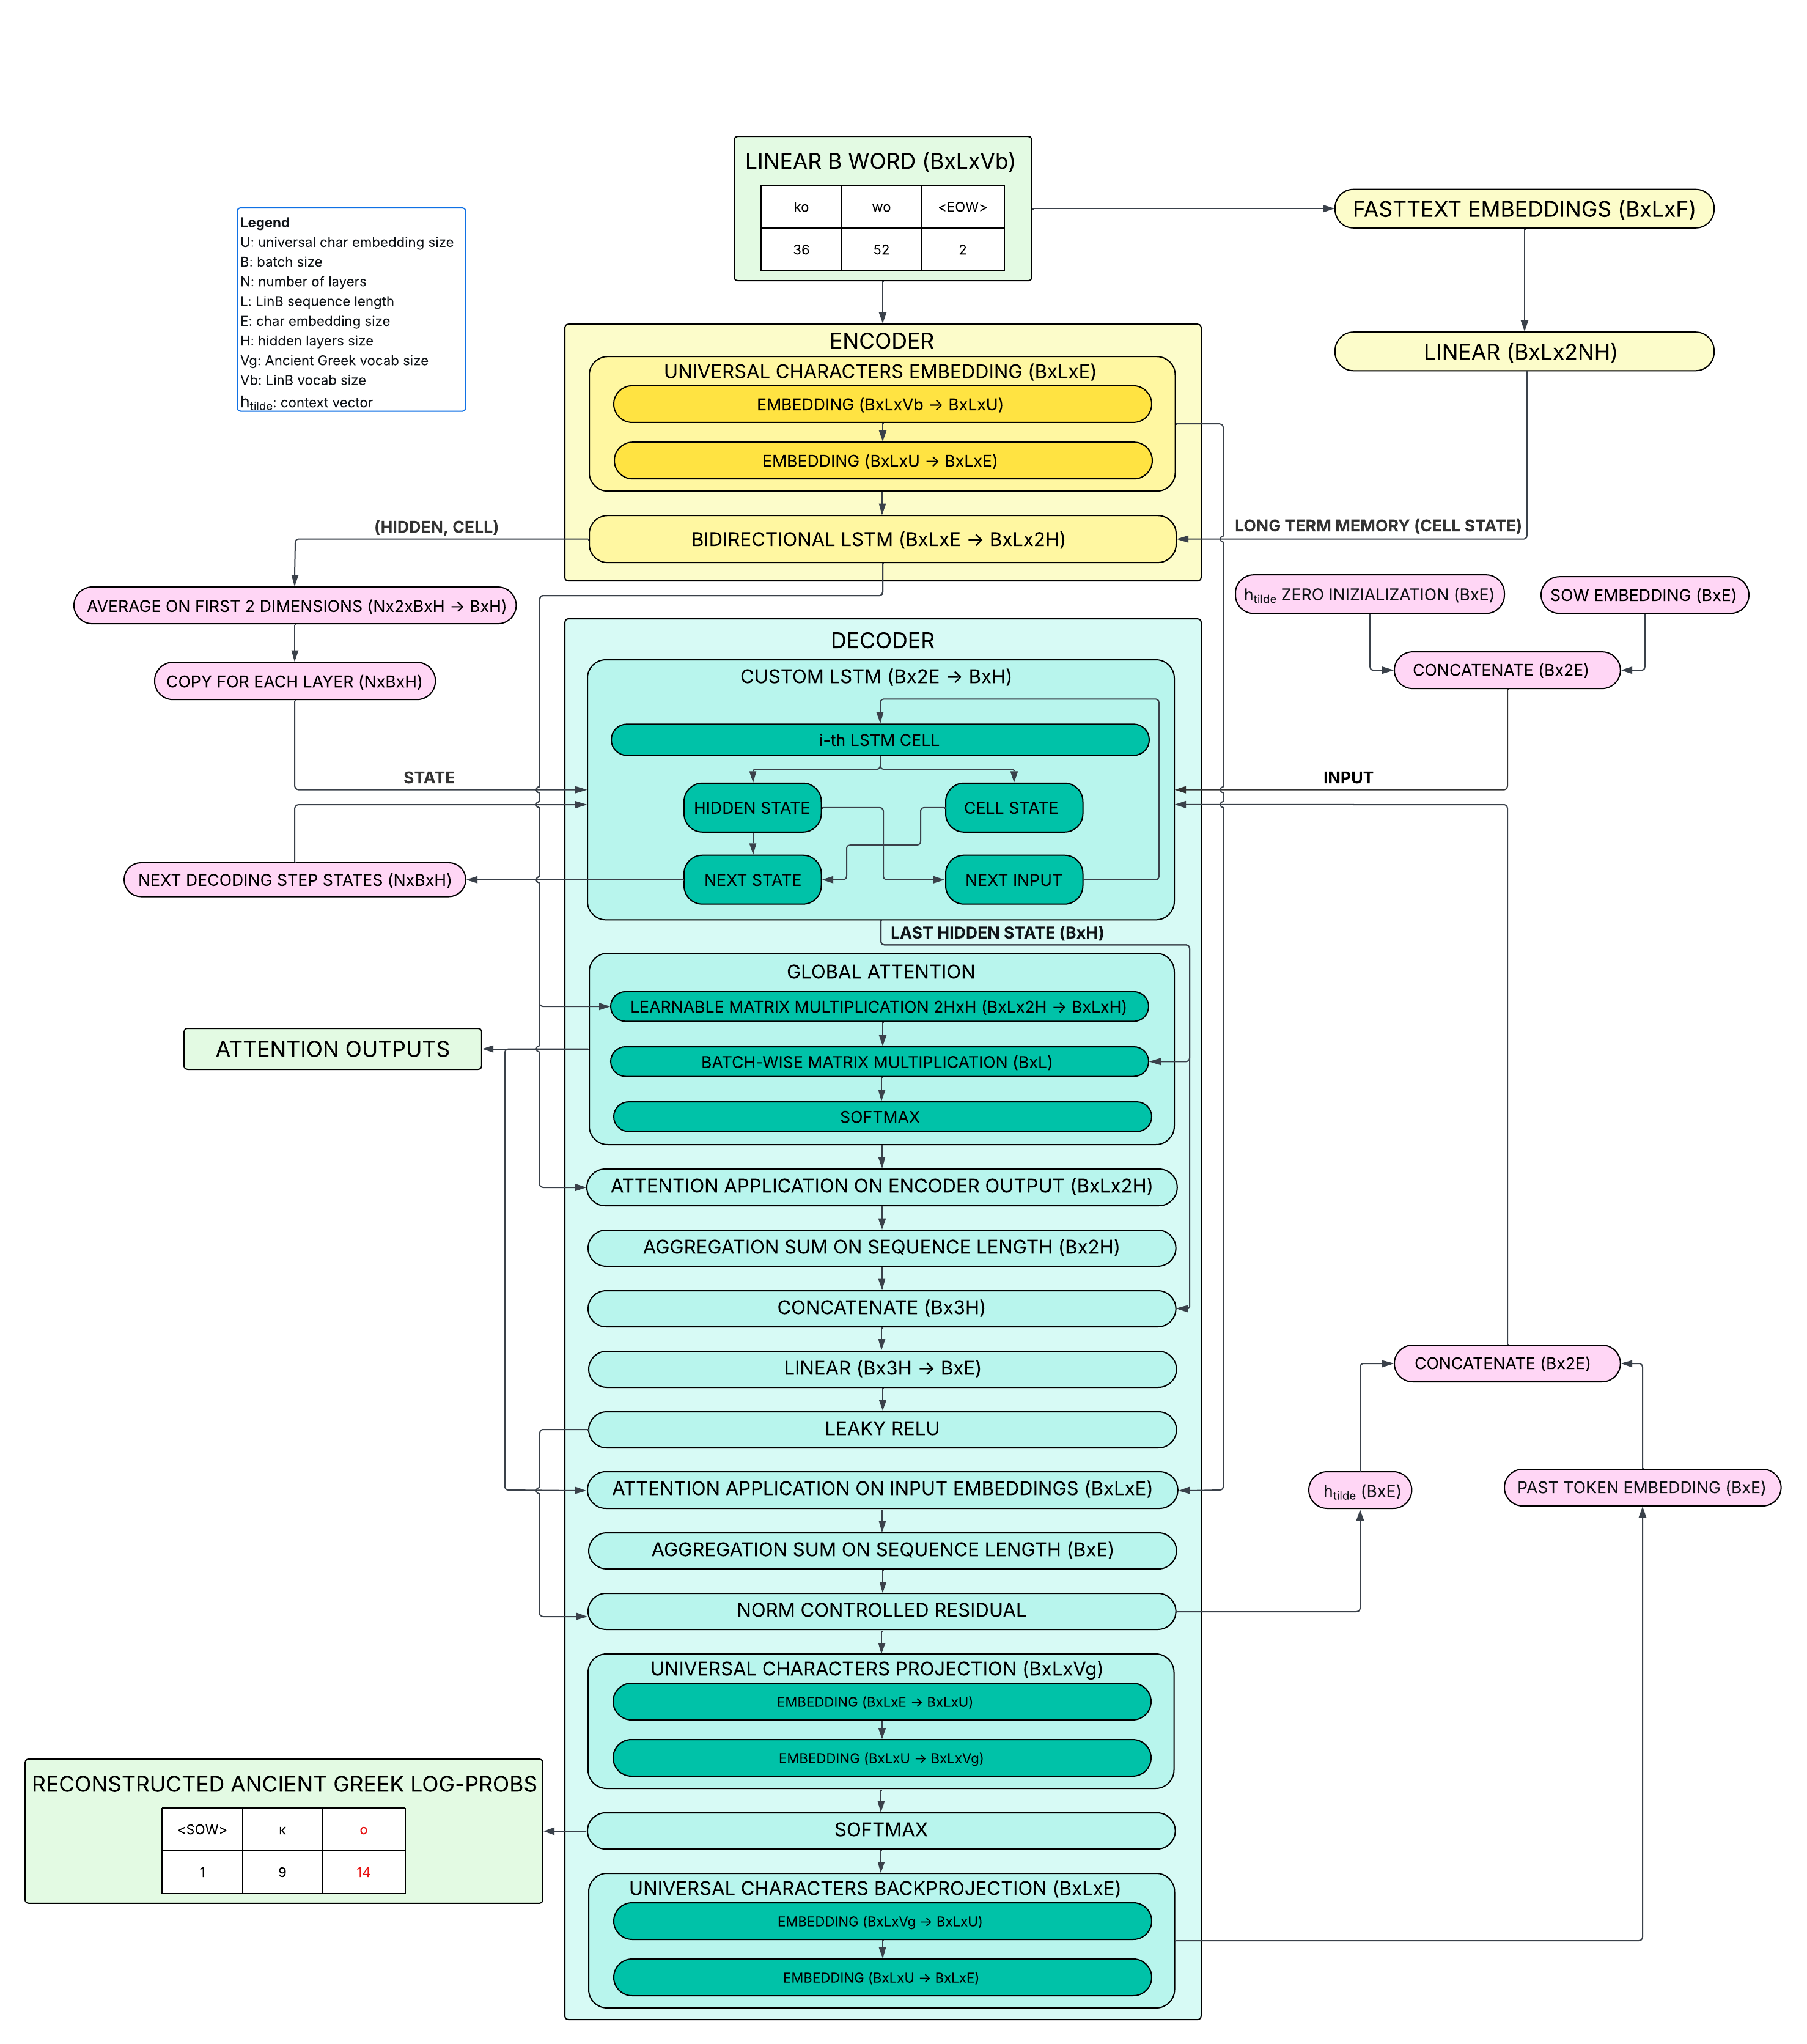
\includegraphics[width=1.2\textwidth]{Images/luo_model.png} % Adjust width and filename
    \caption{Graphical representation of the model architecture.}
    \label{fig:luo_model}
\end{figure}

\begin{figure}[H]
    \centering
    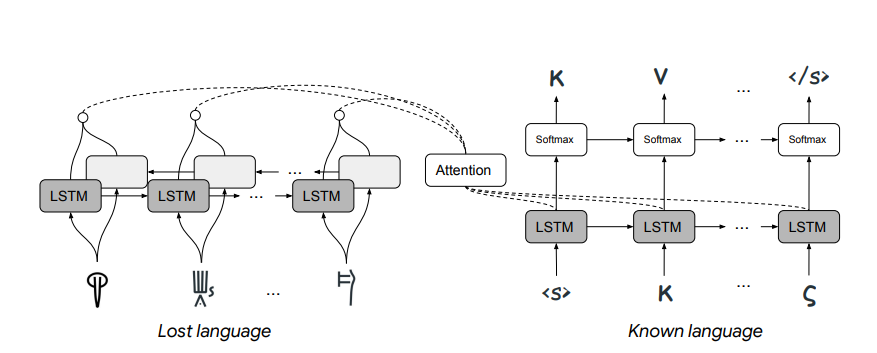
\includegraphics[width=0.8\textwidth]{Images/luo_model_overview.png} % Adjust width and filename
    \caption{Overview of the model architecture.\protect\footnotemark}
    \label{fig:luo_model_overview}
\end{figure}
\footnotetext{Figure \ref{fig:luo_model_overview} prepared by Jiaming Luo.}

\subsection{Output Refinement}
The model supports three output modes.
The first is a corpus-constrained maximum-likelihood selection (MLE) based on the decoder's character distributions.
Given the decoder outputs $\{p_t\}$ for $t=1,\ldots,T_{\max}$, where $p_t\in\mathbb{R}^{V_g}$ is a probability vector over the Greek vocabulary at step $t$, each candidate word $y_j=(y_{j, 1},\ldots,y_{j, T_w})$ in the lexicon is scored by the product of the probabilities of its characters:
\[
\mathbf{P}_{\theta}(y_j \mid x_i)
= \prod_{t=1}^{T_w} p_t[y_{j, t}] \, ,
\]
Equivalently, if $E(y_j)\in\{0,1\}^{T_w\times V_g}$ is the one-hot matrix of $y_j$ (row $t$ is one-hot for $y_{j,t}$), indicating with $E_t(y_j)$ the $t$-th row, then
\[
\log \mathbf{P}_{\theta}(y_j \mid x_i)
= \sum_{t=1}^{T_w} E_t(y_j)\,\log p_t \, ,
\]
which is the form used in practice for numerical stability.

As explained in Section \ref{sec:generative-framework}, the other two output modes are defined via a minimum-cost flow over a bipartite graph.
Edges from source to lost-language nodes have unit capacity; edges from known-language nodes to sink have capacity $C$ (a hyperparameter); the edges between languages have capacity $1$.
The two modes differ only in how the edge costs $d_{ij}$ (from $x_i$ to $y_j$) are computed.

In the first flow mode, set $d_{ij}=-\log \mathbf{P}_{\theta}(y_j\mid x_i)$, i.e., reuse the corpus-constrained MLE score.

In the second flow mode, the character probabilities $\{p_t\}$ are used to sample multiple candidate Ancient Greek words, which are then compared to each lexicon word $y_j$ via normalized edit distance.
For each lost language item $x_i$ we estimate, for every lexicon word $y_j$, an expected normalized edit distance under the decoder's output distributions:

\begin{enumerate}[leftmargin=2em]
\item \textbf{Sample $S$ strings from the decoder.}
Using the per-step character distributions $\{p_t\}_{t=1}^{T_{\max}}$, optionally sharpened by a temperature $\alpha>1$, independently draw $S$ strings and truncate at \textsc{eos}:
$s_{i,k}=(s_{i,k,1},\ldots,s_{i,k,T_{s_{i,k}}})$, $k=1,\ldots,S$.

\item \textbf{Score each sample by its (log-)likelihood.}
With an \textsc{eos} mask $m_{i,k,t}\in\{0,1\}$, define
\[
\log \mathbf{P}(s_{i,k}\!\mid x_i)
\;=\;
\sum_{t=1}^{T_{\max}} m_{i,k,t}\,\log p_t\!\bigl[s_{i,k,t}\bigr].
\]

\item \textbf{Compute normalized edit distances to each candidate.}
For every lexicon word $y_j$ and each sample $s_{i,k}$,
\[
\delta\bigl(y_j,s_{i,k}\bigr)
\;=\;
\frac{\mathrm{Lev}\bigl(y_j,s_{i,k}\bigr)}
     {\min\!\bigl(\lvert y_j\rvert,\lvert s_{i,k}\rvert\bigr)+1}\,.
\]
Also the "original" candidate with zero distance is included:
$\delta\bigl(y_j,s_{i,0}\bigr)\equiv 0$ and score
$\log \mathbf{P}(s_{i,0}\!\mid x_i)\equiv \log \mathbf{P}_{\theta}(y_j\!\mid x_i)$.

\item \textbf{Weight and average.}
Convert the $(1+S)$ log-scores
$\{\log \mathbf{P}(s_{i,k}\!\mid x_i)\}_{k=0}^{S}$
to non-negative weights $\{w_{i,k}\}_{k=0}^{S}$ proportional to their likelihoods and normalized to sum to $1$.
Set the edge cost to the expected normalized edit distance:
\[
d_{ij}
\;=\;
\sum_{k=0}^{S} w_{i,k}\,\delta\bigl(y_j,s_{i,k}\bigr).
\]
\end{enumerate}


\begin{figure}[H]
    \centering
    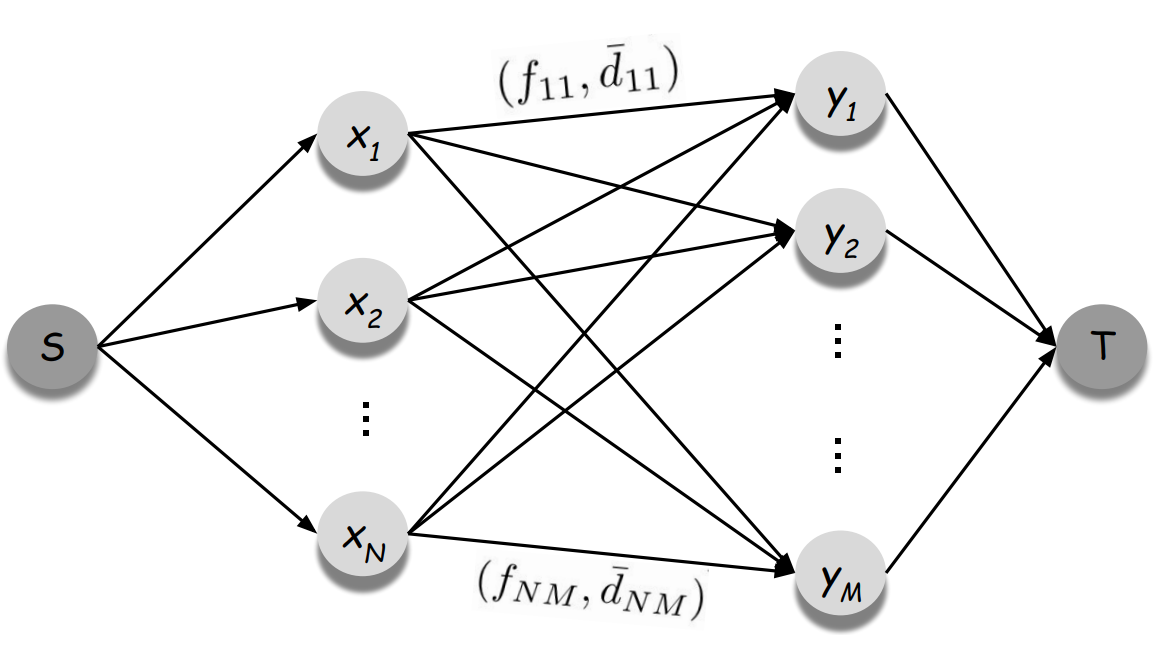
\includegraphics[width=1\textwidth]{Images/luo_flow.png} % Adjust width and filename
    \caption{Overview of the min-cost flow architecture.\protect\footnotemark}
    \label{fig:luo_flow}
\end{figure}
\footnotetext{Figure \ref{fig:luo_flow} prepared by Jiaming Luo.}

\subsection{The loss functions}
The model is trained by minimizing the objective function introduced in Section \ref{sec:generative-framework}.
However, the flow solver returns sparse values, as the flow values for the edges are mostly zeros.
This would likely discard most valid cognate pairs during training.

To address this issue, Luo proposed to use an exponential decay for the flow values in the loss function computation.
These values are updated in each E-step and used in the M-step to compute the loss.
Concretely, the flow values at iteration $\tau$ are updated as follows:
\[
f_{ij}^{(\tau)} \;=\; \gamma\,f_{ij}^{(\tau-1)} + (1-\gamma)\,\tilde{f}_{ij}^{(\tau)} \quad \forall\, i,j,
\]
where $\tilde{f}_{ij}^{(\tau)}$ are the flow values returned by the flow solver at iteration $\tau$, and $\gamma\in[0,1)$ is a hyperparameter that controls the decay rate.

The loss function is then defined as:
\begin{gather*}
\mathcal{L}_{\mathrm{NLL}} =
- \sum_{y_j \in \mathcal{Y}} f_j^{(\tau)} \log \left(\sum_{x_i \in \mathcal{X}} \exp \!\left(\log f_{ij}^{(\tau)} + \log \mathbf{P}_{\theta}(y_j \mid x_i) \right) \right) \;= \\[2pt]
- \sum_{y_j \in \mathcal{Y}} f_j^{(\tau)} \log \left(\sum_{x_i \in \mathcal{X}} f_{ij}^{(\tau)} \cdot \mathbf{P}_{\theta}(y_j \mid x_i) \right) = - \log \left(\prod_{y_j \in \mathcal{Y}} \left( \sum_{x_i \in \mathcal{X}} f_{ij}^{(\tau)} \cdot \mathbf{P}_{\theta}(y_j \mid x_i) \right)^{f_j^{(\tau)}} \right) \, ,
\end{gather*}
where $f_j^{(\tau)} = \sum_{x_i \in \mathcal{X}} f_{ij}^{(\tau)}$ is the aggregated flow into node $y_j$ and acts as a weight for the loss of that word.

An additional loss component is introduced to encourage monotonic alignments.
This component, called monotonic alignment regularization, penalizes unaligned positions of predicted characters.
The loss acts directly on the attention weights $\alpha_t$ produced by the Global Attention module.

Concretely, the attention weights are interpreted, for each word of the lost language $x_i$, as the alignment probability over the input sequence at each decoding step $t$.
Therefore, $\alpha_t^{(i)}(k) = \mathbf{P}(a_t^{(i)}=k \mid x_i)$, where $a_t^{(i)}$ is the alignment position at step $t$ for word $x_i$.
This probability is used to derive the expected alignment position for each character of the output sequence:
\[
pos_t^{(i)} \;=\; \sum_{k=1}^{L} k \cdot \alpha_t^{(i)}(k)
\;=\; \sum_{k=1}^{L} k \cdot \mathbf{P}(a_t^{(i)}=k \mid x_i) \, .
\]
The monotonic alignment regularization loss is then defined as:
\[
\mathcal{L}_{\mathrm{MAR}} \;=\; \sum_{x_i \in \mathcal{X}} \sum_{t=1}^{T_{\max}} \bigl(pos_t^{(i)} - pos_{t-2}^{(i)} - 1\bigr)^2 \, ,
\]
to accommodate the fact that Linear B is a syllabic language and usually one Linear B sign corresponds to two Greek letters.
An example of alignment between a Linear B word and its Ancient Greek cognate is presented in Figure \ref{fig:alignment_example}.
\begin{figure}[H]
    \centering
    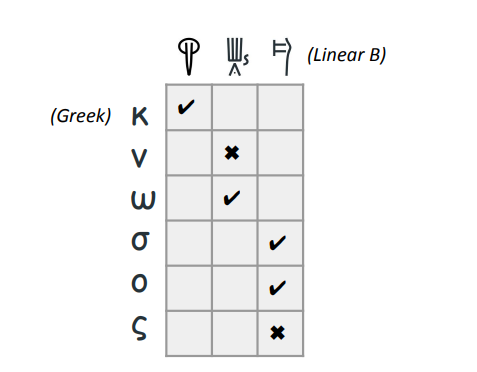
\includegraphics[width=0.6\textwidth]{Images/alignment.png} % Adjust width and filename
    \caption{Example of alignment between a Linear B word and its Ancient Greek cognate. \cmark\ and \xxmark\ indicate correct and incorrect alignment positions, respectively. The misalignment between \textlinb{\Bno} (no) and \textgreek{ν} corresponds to a deletion error, while the misalignment between \textlinb{\Bso} (so) and \textgreek{ς} corresponds to an insertion error.\protect\footnotemark}
    \label{fig:alignment_example}
\end{figure}
\footnotetext{Figure \ref{fig:alignment_example} prepared by Jiaming Luo.}

The final loss function is a weighted sum of the two components:
\[
\mathcal{L} \;=\; \mathcal{L}_{\mathrm{NLL}} + \lambda\,\mathcal{L}_{\mathrm{MAR}} \, ,
\]
where $\lambda$ is a hyperparameter that controls the trade-off between the two loss components.

\subsection{Training Procedure}
As anticipated in Section \ref{sec:generative-framework}, training proceeds in an EM-style loop.
We initialize the alignment flow matrix with a simple prior and then alternate between:

\begin{itemize}[leftmargin=2em]
  \item \textbf{M-step:} fit the seq2seq parameters \(\theta^{(\tau)}\) by maximizing the corpus likelihood under the fixed flows \(f^{(\tau-1)}\).
  \item \textbf{E-step:} recompute edge costs from \(\theta^{(\tau)}\), solve a minimum-cost flow to obtain raw flows \(\tilde f^{(\tau)}\), and update the stable flows via exponential smoothing:
  \[
    f_{ij}^{(\tau)} \;=\; \gamma\,f_{ij}^{(\tau-1)} \;+\; (1-\gamma)\,\tilde f_{ij}^{(\tau)} \, .
  \]
\end{itemize}

To reduce overfitting to the previous iterate and to avoid poor local minima, the neural parameters are re-initialized at the start of each new M-step.
This procedure is summarized in the pseudocode of Algorithm \ref{alg:em-flow}.

This behavior yields distinctive loss/accuracy trajectories for each split (Figure \ref{fig:validation-acc}): curves change sharply at E-M boundaries because flows are recomputed and model parameters are re-initialized.
A practical mitigation is to aggregate within each E-step (e.g., average across its M-steps) or, more conservatively, to report only the final M-step metrics.

The full training procedure and loss computations are graphically illustrated in Figure \ref{fig:luo_framework}.

\begin{figure}[H]
    \centering
    \begin{subfigure}[b]{0.46\textwidth}
        \centering
        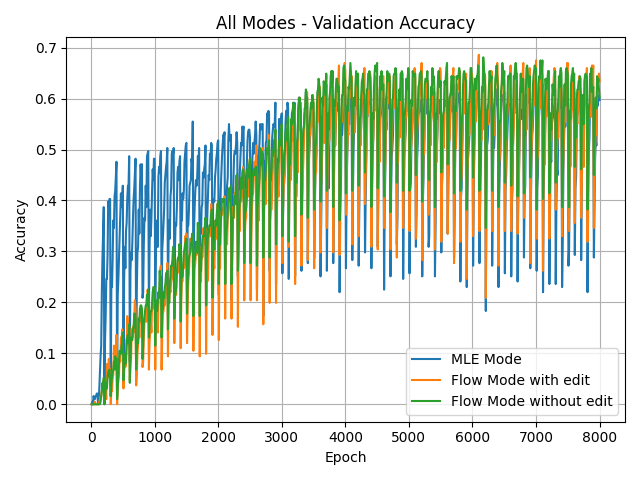
\includegraphics[width=\textwidth]{Images/accuracy_all_modes_validation.png}
        \caption{Accuracy at each M-step.}
        \label{fig:validation-acc-m}
    \end{subfigure}\hfill
    \begin{subfigure}[b]{0.46\textwidth}
        \centering
        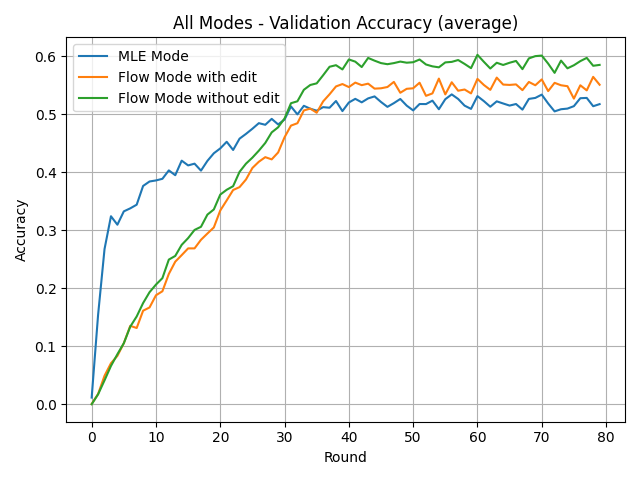
\includegraphics[width=\textwidth]{Images/average_accuracy_all_modes_validation.png}
        \caption{Average accuracy at each E-step.}
        \label{fig:validation-acc-e}
    \end{subfigure}
    \caption{Validation accuracy during training. (a) Raw per M-step accuracy. \\ 
    (b) Accuracy averaged within each E-step.}
    \label{fig:validation-acc}
\end{figure}

\begin{algorithm}[H]
    \SetAlgoNoLine
    \DontPrintSemicolon
    \SetAlgoNoEnd
    
    \SetKwInOut{Input}{Input}
    \SetKwInOut{Output}{Output}
    \SetKwProg{Fn}{Function}{}{}

    \Input{$\mathcal{X}, \mathcal{Y}$ (vocabularies);\ $T$ (number of iterations);\ $N$ (number of cognate pairs to identify)}
    \Output{$f^{(T)}_{ij}$ (final soft alignments/flows)}
    
    \BlankLine
    $f^{(0)}_{ij} \gets \dfrac{N}{|\mathcal{X}|\,|\mathcal{Y}|}$ \tcp*{Initialize uniform flow}
    \For{$\tau \gets 1$ \KwTo $T$}{
        $\theta^{(\tau)} \gets \mathrm{MLE\mbox{-}TRAIN}\!\bigl(f^{(\tau-1)}_{ij}\bigr)$\;
        $d^{(\tau)}_{ij} \gets \mathrm{EDIT\mbox{-}DIST}\!\bigl(x_i, y_j;\, \theta^{(\tau)}\bigr)$\;
        $\tilde f^{(\tau)}_{ij} \gets \mathrm{MIN\mbox{-}COST\mbox{-}FLOW}\!\bigl(d^{(\tau)}_{ij}\bigr)$\;
        $f^{(\tau)}_{ij} \gets \gamma\, f^{(\tau-1)}_{ij} + (1-\gamma)\,\tilde f^{(\tau)}_{ij}$\;
        \textsc{Reset}$\!\bigl(\theta^{(\tau)}\bigr)$\;
    }
    \Return{$f^{(T)}_{ij}$}\;

    \BlankLine
    \Fn{MLE-TRAIN{$\bigl(f^{(\tau)}_{ij}\bigr)$}}{
        $\displaystyle \theta^{(\tau)} \gets \arg\max_{\theta}\ \prod_{y_j\in\mathcal{Y}} \mathbf{P}_{\theta}\!\bigl(y_j \mid \mathcal{X}, \mathcal{F}\bigr)$\;
        \Return{$\theta^{(\tau)}$}\;
    }

    \caption{Iterative training with EM and minimum-cost flow \protect\footnotemark}\label{alg:em-flow}
\end{algorithm}
\footnotetext{Algorithm \ref{alg:em-flow} taken by Jiaming Luo.}

\begin{figure}[H]
    \begin{adjustbox}{center}
        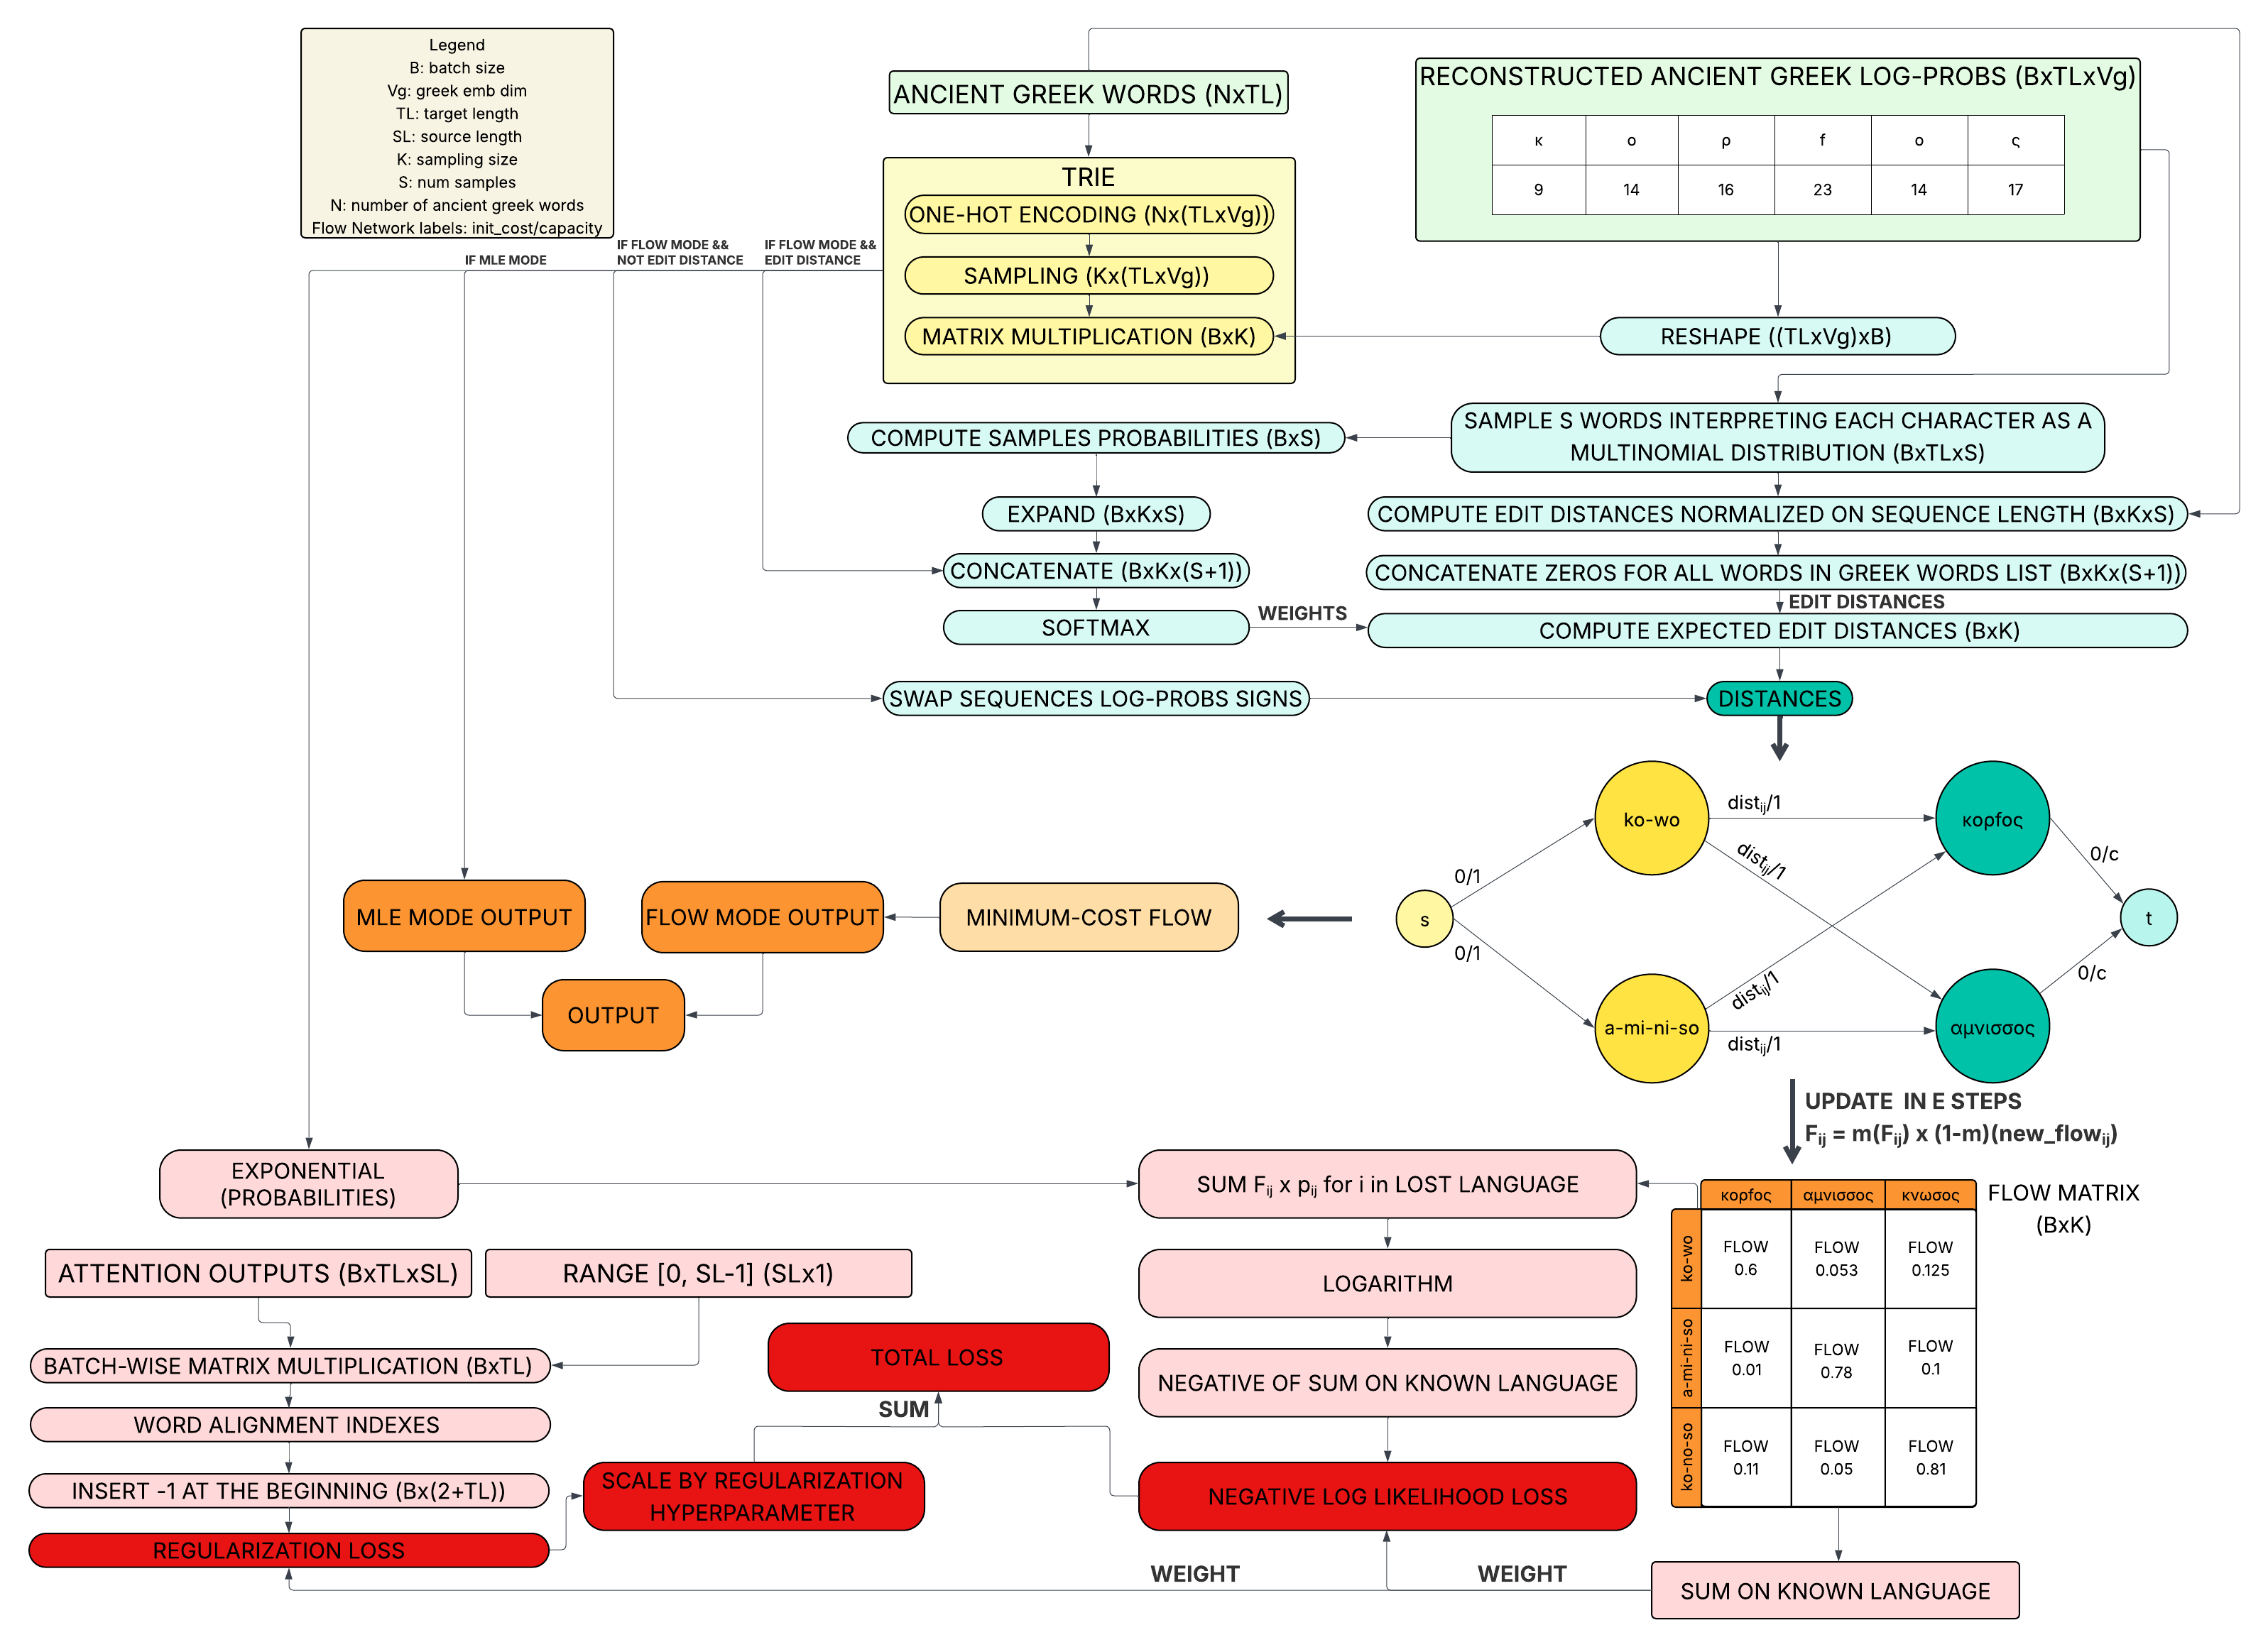
\includegraphics[width=1.25\textwidth]{Images/luo_framework.png}
    \end{adjustbox}
    \caption{Graphical outline of Luo's training procedure.}
    \label{fig:luo_framework}
\end{figure}

\subsection{Results} \label{sec:results}
In this section, I present the results of my experiments with the cognate matching model on three datasets:
\begin{itemize}[leftmargin=2em]
    \item \textbf{Luo's dataset} \cite{luo}, which contains 919 cognate pairs.
    \item \textbf{Luo's corrected dataset}, which contains 976 cognate pairs, obtained by applying some manual corrections on Luo's dataset.
    \item \textbf{Our dataset}, which contains 1911 cognate pairs from both Luo's dataset and Tselentis' \cite{tselentis} dataset, with additional manually identified pairs using the brute-force algorithm, and Ventris and Chadwick's notes \cite{chadwick-notes}.
\end{itemize}

Overall, I ran two sets of experiments.
In the first set, I compared the performance of the model on the full datasets, without defining train/validation/test splits.
In the second set, I defined train/validation/test splits for both Luo's dataset and our dataset, and compared the performance of the model on each split.
The sizes of the splits are the following: 80\% of samples for training, 10\% for validation, and 10\% for test.
For both sets of experiments, I compared the model across all output modes, with and without initializing the LSTM cell states with FastText embeddings.
The results are presented in the tables below.

\begin{table}[h!]
\centering
\begin{tabular}{|c|c|c|c|}
\hline
\textbf{LSTM Initialization} & \textbf{MLE} & \textbf{Flow without edit} & \textbf{Flow with edit} \\
\hline
zero   & 0.830 & 0.831 & 0.781 \\
custom & 0.822 & 0.822 & 0.820 \\
\hline
\end{tabular}
\caption{Comparison of model performance on Luo's original dataset.}
\end{table}

\begin{table}[h!]
\centering
\begin{tabular}{|c|c|c|c|}
\hline
\textbf{LSTM Initialization} & \textbf{MLE} & \textbf{Flow without edit} & \textbf{Flow with edit} \\
\hline
zero   & 0.827 & 0.828 & 0.781 \\
custom & 0.841 & 0.841 & 0.840 \\
\hline
\end{tabular}
\caption{Comparison of model performance on Luo's corrected dataset.}
\end{table}

\begin{table}[h!]
\centering
\begin{tabular}{|c|c|c|c|}
\hline
\textbf{LSTM Initialization} & \textbf{MLE} & \textbf{Flow without edit} & \textbf{Flow with edit} \\
\hline
zero   & 0.694 & 0.711 & 0.671 \\
custom & 0.662 & 0.662 & 0.672 \\
\hline
\end{tabular}
\caption{Comparison of model performance on our dataset.}
\end{table}

It can be observed that, despite the stabilization effect of the custom LSTM initialization, when the model converges with a zero initialization it achieves better performance.
Particularly, the model attains higher accuracy on our more challenging and extensive dataset, reaching 71.1\% with the flow without edit mode.
The final accuracy and loss at each E-step during training on our dataset with zero initialization of the cell states are presented in Figure \ref{fig:acc-loss-all}.

\begin{figure}[H]
    \centering
    \begin{subfigure}[b]{0.46\textwidth}
        \centering
        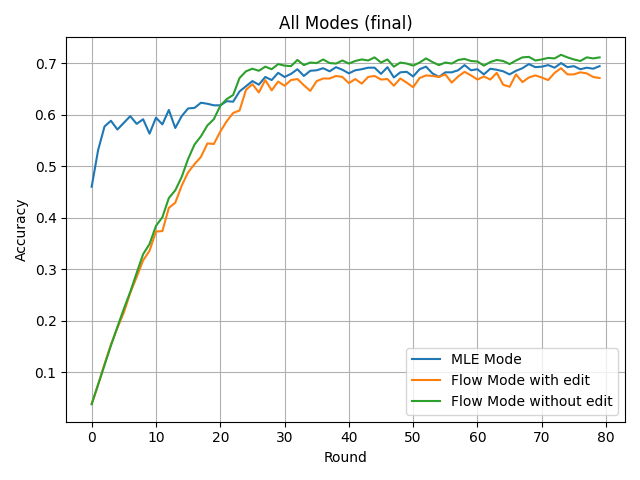
\includegraphics[width=\textwidth]{Images/final_accuracy_all_modes.png}
        \caption{Final accuracy at each E-step.}
        \label{fig:final-acc-all}
    \end{subfigure}\hfill
    \begin{subfigure}[b]{0.46\textwidth}
        \centering
        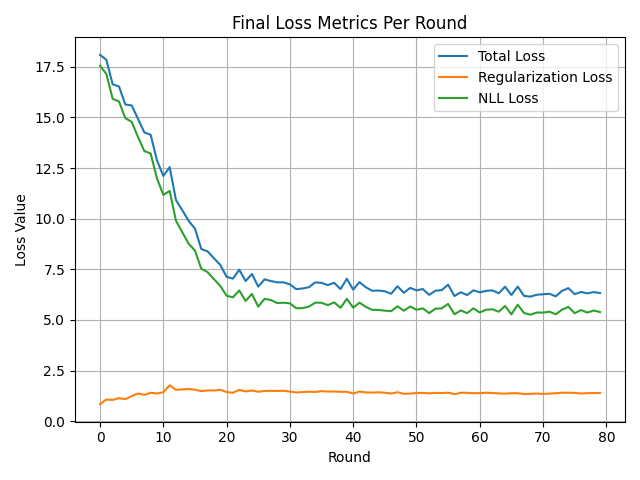
\includegraphics[width=\textwidth]{Images/final_loss_all_metrics.png}
        \caption{Final loss at each E-step.}
        \label{fig:final-loss-all}
    \end{subfigure}
    \caption{Metrics for the zero-initialized model during training on our dataset. \\
    (a) Accuracy. (b) Loss.}
    \label{fig:acc-loss-all}
\end{figure}

The same trends are observed in the experiments with train/validation/test splits.
However, due to the reduced size of the training set and the removal of some cognate pairs from it, the overall performance is lower.
While the zero-initialized model remains strong, the custom-initialized variant degrades substantially.
The results are presented in the tables below.

\begin{table}[h!]
\centering
\begin{tabular}{|c|c|c|c|c|}
\hline
\textbf{LSTM Init} & \textbf{Split} & \textbf{MLE} & \textbf{Flow w/o edit} & \textbf{Flow w/ edit} \\
\hline
\multirow{3}{*}{zero}
& Train      & 0.789 & 0.790 & 0.735 \\
& Validation & 0.663 & 0.674 & 0.696 \\
& Test       & 0.761 & 0.761 & 0.728 \\
\hline
\multirow{3}{*}{custom}
& Train      & 0.411 & 0.423 & 0.435 \\
& Validation & 0.391 & 0.424 & 0.435 \\
& Test       & 0.359 & 0.359 & 0.435 \\
\hline
\end{tabular}
\caption{Performance (Train/Validation/Test) on Luo's original dataset.}
\end{table}

\begin{table}[h!]
\centering
\begin{tabular}{|c|c|c|c|c|}
\hline
\textbf{LSTM Init} & \textbf{Split} & \textbf{MLE} & \textbf{Flow w/o edit} & \textbf{Flow w/ edit} \\
\hline
\multirow{3}{*}{zero}
& Train      & 0.782 & 0.785 & 0.732 \\
& Validation & 0.717 & 0.717 & 0.663 \\
& Test       & 0.739 & 0.739 & 0.696 \\
\hline
\multirow{3}{*}{custom}
& Train      & 0.457 & 0.469 & 0.486 \\
& Validation & 0.446 & 0.467 & 0.511 \\
& Test       & 0.370 & 0.380 & 0.511 \\
\hline
\end{tabular}
\caption{Performance (Train/Validation/Test) on Luo's corrected dataset.}
\end{table}

\begin{table}[h!]
\centering
\begin{tabular}{|c|c|c|c|c|}
\hline
\textbf{LSTM Init} & \textbf{Split} & \textbf{MLE} & \textbf{Flow w/o edit} & \textbf{Flow w/ edit} \\
\hline
\multirow{3}{*}{zero}
& Train      & 0.645 & 0.658 & 0.639 \\
& Validation & 0.597 & 0.602 & 0.634 \\
& Test       & 0.625 & 0.646 & 0.646 \\
\hline
\multirow{3}{*}{custom}
& Train      & 0.238 & 0.275 & 0.367 \\
& Validation & 0.262 & 0.262 & 0.377 \\
& Test       & 0.224 & 0.234 & 0.370 \\
\hline
\end{tabular}
\caption{Performance (Train/Validation/Test) on our dataset.}
\end{table}

This significant drop in the custom-initialized runs is consistent with a loss–accuracy divergence caused by a representation mismatch.
FastText injects word-level semantic priors into a character-mapping task.
As a result, the model becomes confidently wrong on many instances: the negative log-likelihood can keep improving (higher confidence), while accuracy on held-out data declines (worse argmax decisions).
In short, the initialization biases the decoder toward signals that are orthogonal to the target grapheme-level correspondences, leading to miscalibration and poorer generalization, due to representational mismatch.

The final accuracy of all splits, using MLE mode, and the final accuracy of the test split, using all output modes, of the zero-initialized model during training on our dataset are presented in Figure \ref{fig:acc-loss-splits}.
\begin{figure}[H]
    \centering
    \begin{subfigure}[b]{0.46\textwidth}
        \centering
        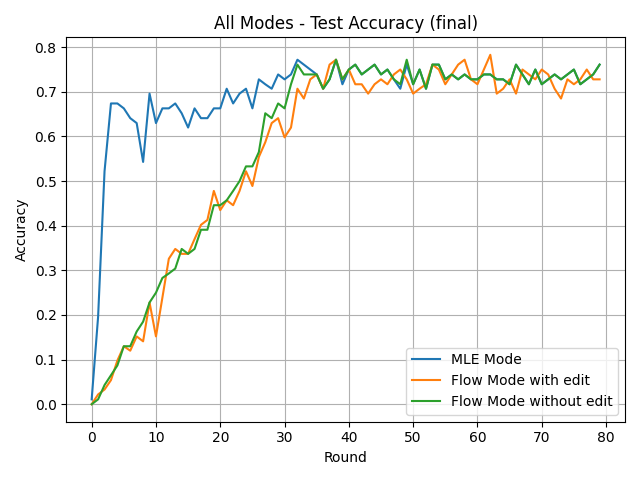
\includegraphics[width=\textwidth]{Images/final_accuracy_all_modes_test.png}
        \caption{Final accuracy at each E-step for the test set in all modes.}
        \label{fig:final-acc-test-all}
    \end{subfigure}\hfill
    \begin{subfigure}[b]{0.46\textwidth}
        \centering
        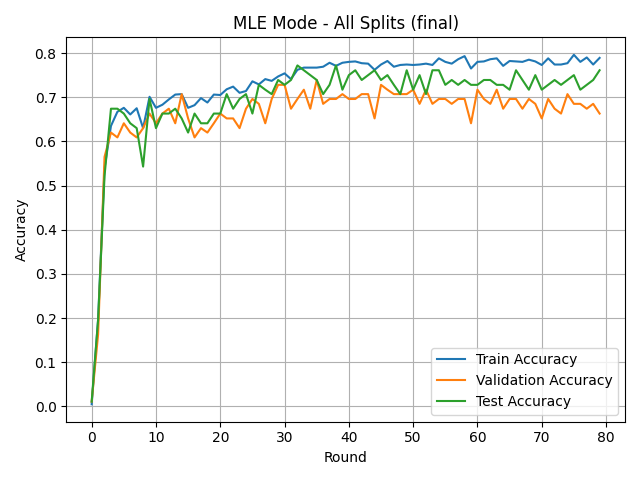
\includegraphics[width=\textwidth]{Images/final_accuracy_mle_mode_all_splits.png}
        \caption{Final accuracy at each E-step in MLE mode for all splits.}
        \label{fig:final-acc-mle-all}
    \end{subfigure}
    \caption{Metrics for the zero-initialized model during training on our dataset. \\ 
    (a) Accuracy for the test set in all modes. (b) Accuracy in MLE mode for all splits.}
    \label{fig:acc-loss-splits}
\end{figure}
\chapter{Auxialiary Classifiers}
PALLE

\backmatter
\cleardoublepage
\phantomsection % Give this command only if hyperref is loaded
\addcontentsline{toc}{chapter}{\bibname}
% Here put the code for the bibliography. You can use BibTeX or
% the BibLaTeX package or the simple environment thebibliography.

\printbibliography

\end{document}